\documentclass[]{final_report}
\usepackage{graphicx}
\usepackage{hyperref}
\usepackage{float}
\usepackage{longtable}

%%%%%%%%%%%%%%%%%%%%%%
%%% Input project details
\def\studentname{Wing Kiu Lo}
\def\reportyear{Year 3}
\def\projecttitle{An extendible clustering package for Bioinformatics }
\def\supervisorname{Dr Ilia Nouretdinov}
\def\degree{BSc (Hons) in Computer Science and Mathematics}
\def\fullOrHalfUnit{Full Unit} % indicate if you are doing the project as a Full Unit or Half Unit
\def\finalOrInterim{Final Report} % indicate if this document is your Final Report or Interim Report
\def\coursecode{CS3821 Full unit project}

\begin{document}

\maketitle

%%%%%%%%%%%%%%%%%%%%%%
%%% Declaration

\chapter*{Declaration}

This report has been prepared on the basis of my own work. Where other published and unpublished source materials have been used, these have been acknowledged.

\vskip3em

Word Count: 12087

\vskip3em

Student Name: \studentname

\vskip3em

Date of Submission: 25th March 2022

\vskip3em

Signature: Winkie Lo

\newpage

%%%%%%%%%%%%%%%%%%%%%%
%%% Table of Contents
\tableofcontents\pdfbookmark[0]{Table of Contents}{toc}\newpage

%%%%%%%%%%%%%%%%%%%%%%
%%% Your Abstract here

\begin{abstract}

This paper is the final report for a Java-based extendible clustering package for bioinformatics.

An open source application that provides an extendible framework for parsing biological data like FASTA and CSV (DNA Expression Microarrays data) via sequence alignment, clustering algorithms like k-means and hierarchical, and simple visualisation techniques like dendrogram and heatmap. It provides a general foundation for developing bioinformatics applications efficiently in the Java programming language. 


Java 8 is now the minimum supported version for this package and is offered freely under the MIT licence agreement.

By combining reports from various aspects, such as a biological overview of the problem, a detailed description of the implementation of the plugin-architecture, professional issues, and comprehensive documentation on how to extend the program, the purpose of this report is to correctly document both the software engineering and package development procedures used throughout the project.

Users, particularly contributors who want to enhance the project, will benefit from this paper.

\end{abstract}
\newpage

%%%%%%%%%%%%%%%%%%%%%%
%%% Project Spec

\chapter*{Project Specification}
\addcontentsline{toc}{chapter}{Project Specification}

\textbf{An extendible clustering package for bioinformatics}

\paragraph{Aims}
To design and implement an application for clustering different biological data sets with different algorithms using the Java plug-in technology.

\paragraph{Background}
Bioinformatics is currently a quickly growing field within the Computer Science ecosystem. The advent of new sequencing technologies along with the high amount of funding devoted to research in life sciences, have produced a huge amount of biological data which waits to be analysed.\\
Clustering is a technique which is often used for such analysis:  \begin{enumerate}
 \item given a set of elements (protein sequences, gene expression profiles, etc),
 \item performing a clustering amounts to finding meaningful groups in the data set.
\end{enumerate}
 There are different clustering algorithms, each one with different features: 
\begin{enumerate}
 \item hierarchical/non- hierarchical,
 \item overlapping/non-overlapping,
 \item graph-based, etc.
\end{enumerate}
 Also, for different biological data sets, some clustering algorithms are more appropriate than others. \\
 Finally, once a clustering has been obtained there are different techniques to assess the validity of the groupings.

 \textbf{Requirement: } 
In this project a clustering environment for bioinformatics should be developed using the Java language.\\
The environment should be as generic as possible, with a very important feature: it should allow for future extensions.\\
Namely, it should be extendible in three ways:
\begin{enumerate}
 \item New biological data types
 \item New clustering algorithms
 \item New techniques for the visualisation or assessment of the clusters
\end{enumerate}
In order to do that, the Java plugin architecture should be used. This will allow other people to write future extensions to this system, without the need of rewriting its kernel.\\
Thus, the project should be carefully designed and should contain enough generality to prevent further modifications and allow any future plugins to be added to it.\\
The final aim of the project is to produce a solid piece of software which will be made available to the scientific community. It is possible that this work will lead to a publication in a bioinformatics journal.

\textbf{Early Deliveries: } \\
Proof of concept programs: parsers for biological databases, \\
Proof of concept programs: implementation of one clustering algorithm,\\
Proof of concept programs: design of an interface.\\
Reports: Biological databases.\\
Reports: Clustering algorithms.\\
Reports: Design Patterns in Java (mainly plugin architecture).\\

\textbf{Final Deliveries: } \\
The software should be able to work with at least two kind of biological data (micro-array data and sequence data) and two clustering algorithms (for instance k-means and hierarchical clustering). \\
At least one visualisation/assessment technique should be added (for example, over- representation analysis).\\
The report should include a biological overview of the problem,\\
The report should include a detailed description of the implementation of the plugin-architecture, \\
The report should include a comprehensive documentation on how to extend the program.\\

\textbf{Suggested Extensions: }\\
Adding the possibility of processing more biological data (PPI data, for example, CSV, etc)\\
Adding more clustering algorithms, possibly using the Facade pattern with existing implementations (SCSP, Cluster ONE, ...).\\
Developing cluster visualisation techniques: MDS visualisation, dendrograms, etc.\\


%%%%%%%%%%%%%%%%%%%%%%
%%% Introduction
\chapter{Introduction}
This chapter is aim to introduce the aims, goals and objective of the project, the motivation behind the program as well as an overview for the structure of the report. Let's begin with a basic description of the term "Bioinformatics."

\section{The problems}
Bioinformatics is a field that combines knowledge from biology, life science, mathematics, and computer science to derive biological understanding from massive volumes of data~\cite{zhang2009machine}.

The never-ending torrent of data in a world of limited time, drowning in data and fast change, with the explosion of datasets awaiting analysis, numerous bio applications try to automate the process of learning unlabelled data for bioinformatics practitioners, with BioPearl, BioPython, BioJava, and BioWeka being some of the most popular~\cite{gewehr2007bioweka}.
The above list of applications demonstrates that the bioinformatics' field is today regarded as a relatively rich ecosystem, thanks to the open source community's contributions.

Previous programs emphasised acquiring as many possibilities as possible. BioJava, for example, is a well-established framework with limited clustering algorithm possibilities.~\cite{lafita2019biojava}. On the other hand, as a Weka extension project, which is a data mining framework, has more clustering methods, such as simple k means and expectation maximisation clustering. Bioweka, on the other hand, only works with Weka 3.4.19 and Bioweka 0.7.0, and the Java documentation is out of date, making it difficult for users.~\cite{gewehr2007bioweka}. 

For applications that primarily focus on clustering unlabelled biological data in Java, there are few choices. In order to understand how to execute a simple task, such as parsing data, bioinformaticians may be required to study the whole documentation of a well-established system. As a result, an extendible clustering package with visualisation is developed and made accessible to the scientific community, with a focus on users who want to use it especially on unlabelled biological data, with a modern library, simpler interface, fewer lines of coding needed and less confusion. 

\section{Aims and Goals of the project} \label{1.1}

During the COVID-19 pandemic, bioinformatics provided several crucial methods to help scientists understand the virus structure, the similarities between SARS-CoV-2 and SARS-CoV, and much more. Bioinformatics puts vaccine development on a high growth trajectory, and this technique is still evolving at a rapid pace~\cite{ma2021comprehensive}. 

Ideally, the project should be able to parse different biological data file formats such as FASTA, FASTAQ, CSV, GenBank...~\cite{appliedbioinfomatics2019} that contains different data type such as (nucleic acid, genome, protein) sequence, microarray... retrieving the data needed, providing different clustering algorithms and visualising the data with options such as clustered heat-map, dendrogram...

Alternatively, we are aiming to find a pattern or different clusters within an unlabelled dataset using clustering techniques in bioinformatics area such that it would be more effectively to identifies similarity or dissimilarity within data for biologists.

\section{Motivation} \label{1.3}
The primary motivation for developing this project is to be able to deliver software that is potentially valuable to the scientific community by simplifying a task frequently done by bioinformaticians.

From a personal aspect, working on a topic of personal interest and having the chance to learn more about it in depth is an incredible experience.

As a developer, it is important to show that they have the ability to work as a team as well as work independently. By successfully completing this project, it provides an opportunity to demonstrate not only the capacity to work independently but also the ability to work within a strict time frame. Additionally, it gives an opportunity for computer scientists to submit a project to a supervisor in order to simulate a real work environment prior to entering the industry. Furthermore, it may be considered as a personal portfolio for future employment opportunities.

In conclusion, this project introduces a programmer to a significant amount of the software engineering process and allows for the acquisition of new technologies. All of which provide significant motivation from an academic and professional perspective.

\section{Objectives}

In order to meet the project's aims and goals, it will be necessary to create a variety of data parsers, clustering methods, and visualisation techniques.

From the beginning to the end, the software has been written in Java with a minor fraction of Python to improve the visualisation results. The work was documented so the software would be straightforward to use, more robust, and easy to maintain by other bioinformatician or computer scientist in the scientific community, and it is hoped that it will contribute to new and better information for the bio-industry.

\section{Why Java}
There are several bioinformatics projects available in various programming languages, with R, Perl, and Python being one of the most popular~\cite{gewehr2007bioweka}.

As an extendible clustering package, it is critical for users to be able to download and operate the program without having to worry about any potential viruses, as well as the ability to run the application on a variety of different environments and operating systems, among other requirements~\cite{schildt2019java}.

\subsection{Portability}
There are multiples of different environments and operating systems available. Java, on the other hand, runs on a broad range of CPUs, operating systems, and browsers due to its portability allowing the program to run on many different computers~\cite{schildt2019java}.

The Java Virtual Machine which is included in the Java Run Environment converts Java bytecode into machines language. As a result allowing Java to be a platform independent language~\cite{schildt2019java}.

\subsection{Security}
As JVM manages the execution of the java source code, Java prevents viruses from accessing other sections of the computer by isolating the application to the Java execution environment~\cite{schildt2019java}.

\subsection{Object Oriented}
Java is object-oriented and is known for its encapsulation, polymorphism, and inheritance.

\paragraph{Encapsulation} is a method that keeps code and the data it manipulates secure from outside influence and misuse by tying them together. This becomes useful for the BLOSUM class as an example. The class itself is set to be public. However, the matrix class is set to be private, applying restrictions on accessibility, and the double array matrix value is set to be final, applying restrictions to the class, so the value itself cannot be changed. Setting a class to final will make it immutable even for its child class. This leads to inheritance.

\paragraph{Inheritance}An object may inherit the properties of another via the process of inheritance, allowing a child class to inherit traits from its parent class. In this project, class BLOSUM (extends) inherits from class ScoringMatrix, an example of inheritance that allows a wide variety of scoring matrix, such as PAM, for users to extend to the scoring matrix class as an additional extension.

\paragraph{Polymorphism} is the trait that enables a single interface to conduct a broad variety of functions, such as allowing the BLOSUM class to share the matrix format of the ScoringMatrix class with its own values.

\begin{figure}[H]
    \centering
    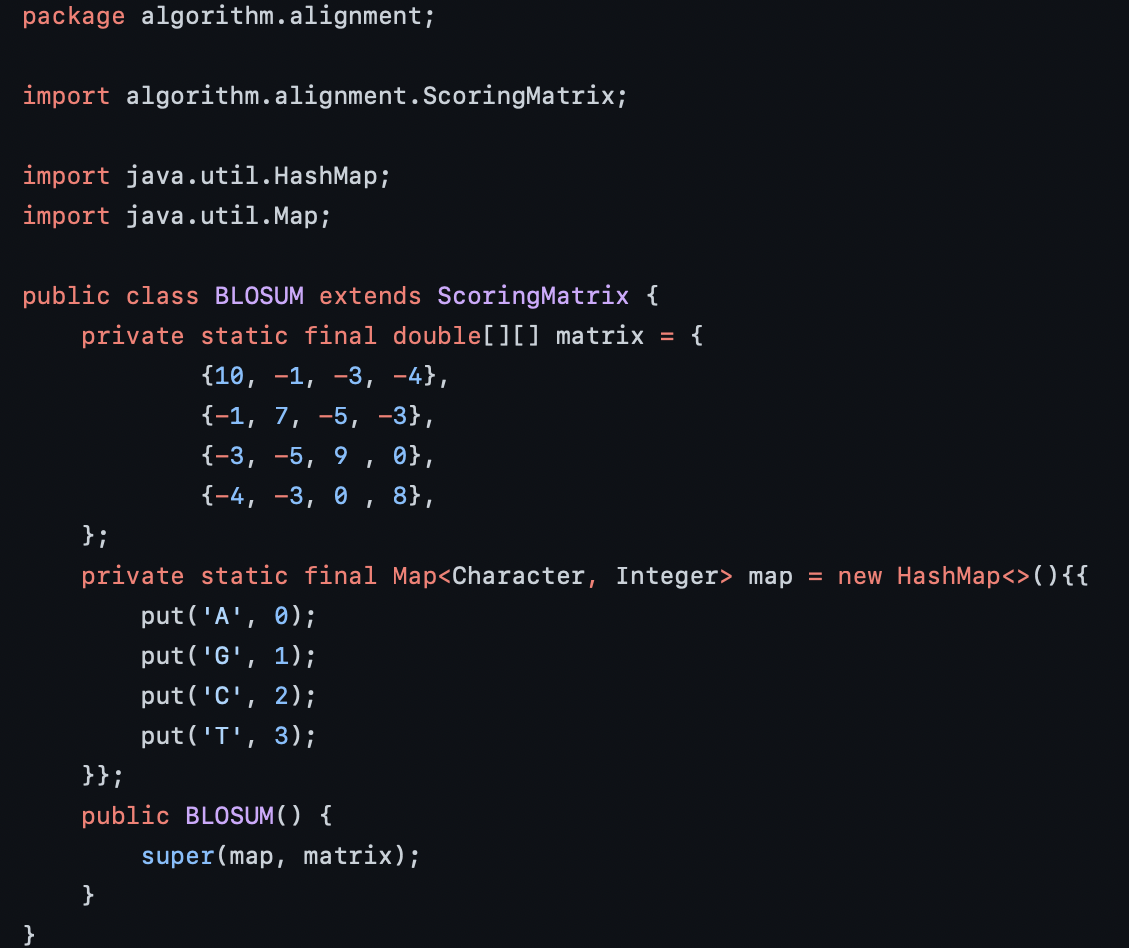
\includegraphics[width=0.5\textwidth]{BLOSUM.png}
    \caption{BLOSUM class}
    \label{fig:BLOSUM_C}
\end{figure}

\begin{figure}[H]
    \centering
    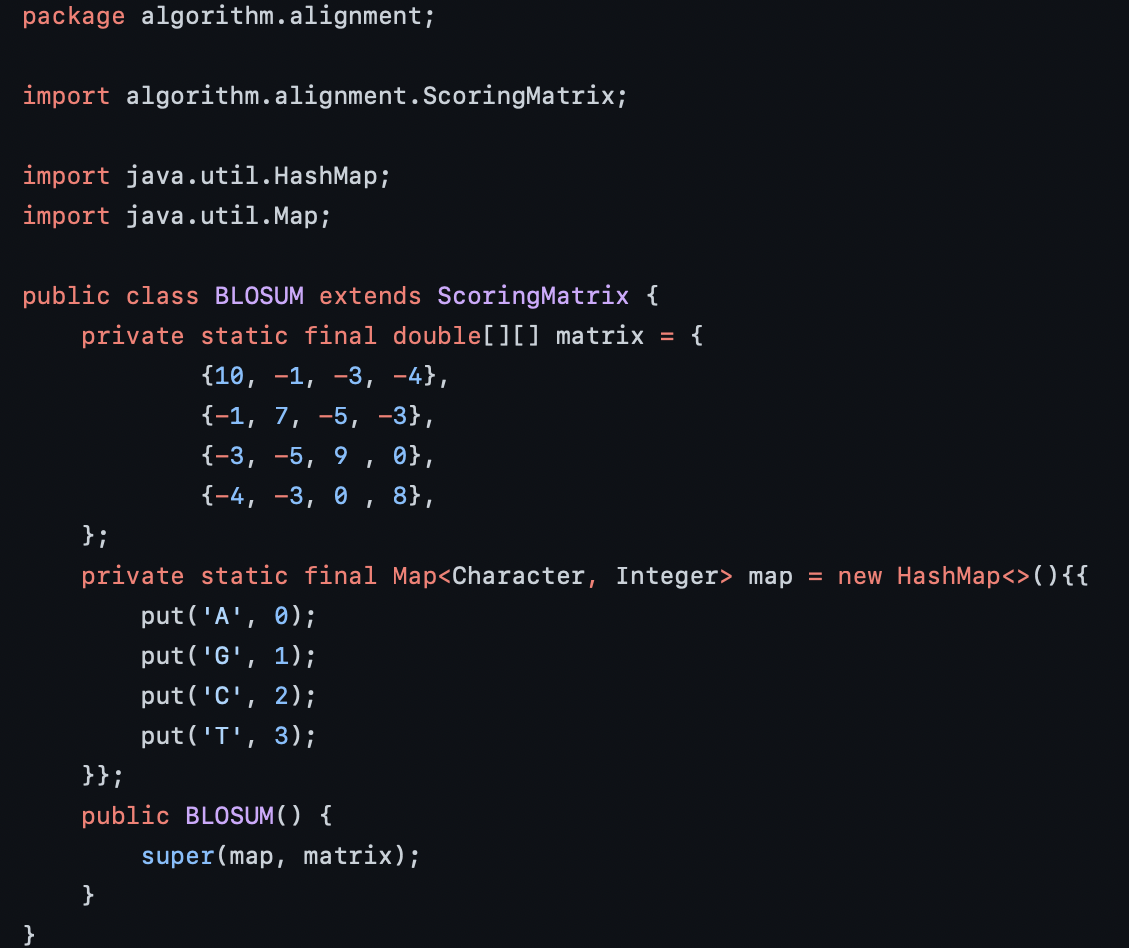
\includegraphics[width=0.5\textwidth]{Scoring Matrix.png}
    \caption{Scoring Matrix class}
    \label{fig:Scoring_Matrix_C}
\end{figure}
As the advantages mentioned above, portable, object-oriented, and secure are the main reasons for choosing Java as the programming language for the project.
The figure below illustrates the other significant aspects that contribute to the ultimate shape of the language~\cite{schildt2019java}.


\begin{figure}[H]
    \centering
    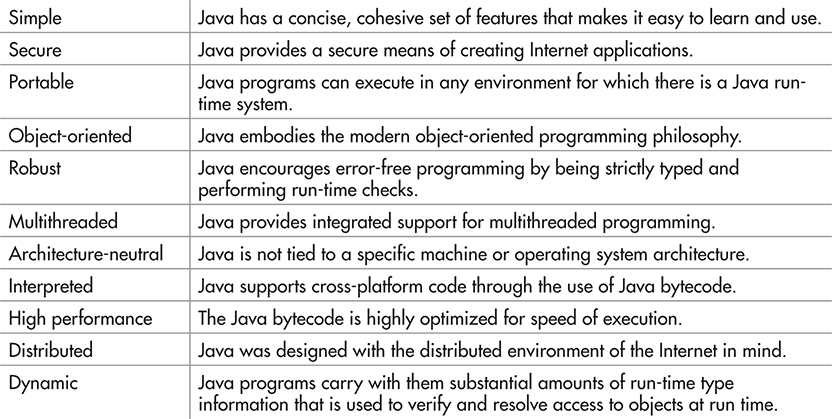
\includegraphics[width=0.5\textwidth]{why java.jpeg}
    \caption{Java buzzwords\cite{schildt2019java}}
    \label{fig:java_buzzwords}
\end{figure}

\section{Milestone}
The goal of this chapter is to demonstrate the report's and project's milestones.
Milestones are necessary for visualising and verifying progress in terms of achievement. It may be used as a checklist to ensure that the project or report satisfies all of the necessary requirements.

\subsection{Reports}
This section concentrates on displaying the detailed reports that have been established. The following is a summary of these reports.
\begin{table}[H]
\resizebox{\textwidth}{!}{%
\begin{tabular}{|lc|}
\hline
\multicolumn{2}{|c|}{\textbf{Milestone}} \\ \hline
\multicolumn{1}{|c|}{\textbf{Item}} &
  \textbf{Description} \\ \hline
\multicolumn{1}{|l|}{Biological Overview Report} &
  \begin{tabular}[c]{@{}c@{}}A document that describes the biological overview of the problem\\ including both the biological and mathematical background theory.\end{tabular} \\ \hline
\multicolumn{1}{|l|}{Software Engineering Report} &
  \begin{tabular}[c]{@{}c@{}}A document that includes a detailed description of the implementation of \\ the plugin-architecture with UML Class diagram, explaining the software engineering methods.\end{tabular} \\ \hline
\multicolumn{1}{|l|}{Instruction Report} &
  \begin{tabular}[c]{@{}c@{}}A document that serves as a comprehensive documentation on \\ how to extend the program with requirements and denpendencies.\end{tabular} \\ \hline
\multicolumn{1}{|l|}{Professional Issues Report} &
  \begin{tabular}[c]{@{}c@{}}A document that breifly explain the professional issues that \\ raised concern throughout the project.\end{tabular} \\ \hline
\multicolumn{1}{|l|}{Analysis Report} &
  \begin{tabular}[c]{@{}c@{}}A document that discuss the critical analysis of the project such as \\ the project's achievements, evidence of reflection, technical decision making \\ and its challenges.\end{tabular} \\ \hline
\multicolumn{1}{|l|}{Architecture Report} &
  \begin{tabular}[c]{@{}c@{}}A document that describes the proof of concept with \\ project information and rules.\end{tabular} \\ \hline
\end{tabular}%
}
\end{table}
\subsection{Programs}
This section focuses on several functions available in the source code as well as the testing package.
\subsection{Source}
\begin{table}[H]
\resizebox{\textwidth}{!}{%
\begin{tabular}{|lc|}
\hline
\multicolumn{2}{|c|}{\textbf{Milestone}}                                                                                  \\ \hline
\multicolumn{1}{|c|}{\textbf{Item}} & \textbf{Description}                                                                \\ \hline
\multicolumn{1}{|l|}{Parsers}       & A package that parse both the sequence and microarray data in FASTA and CSV format. \\ \hline
\multicolumn{1}{|l|}{Alignment}     & A package that provides global alignment with scoring matrix.                       \\ \hline
\multicolumn{1}{|l|}{Clustering} &
  \begin{tabular}[c]{@{}c@{}}A package that includes different distance matrix and linkage with \\ k-means and agglomerative clustering algorithmns.\end{tabular} \\ \hline
\multicolumn{1}{|l|}{Dimension} &
  \begin{tabular}[c]{@{}c@{}}A package that transform microarray data from \\ n-dimension into two-dimensional double arrays\\ using principal component analysis\end{tabular} \\ \hline
\end{tabular}%
}
\end{table}
\subsection{Testing}

\begin{table}[H]
\resizebox{\textwidth}{!}{%
\begin{tabular}{|lc|}
\hline
\multicolumn{2}{|c|}{\textbf{Milestone}}                   \\ \hline
\multicolumn{1}{|c|}{\textbf{Item}} & \textbf{Description} \\ \hline
\multicolumn{1}{|l|}{K Means Test} &
  \begin{tabular}[c]{@{}c@{}}A unit test that displays the visualisation of microarray data using k-means.\\ (scatter plot)\end{tabular} \\ \hline
\multicolumn{1}{|l|}{Sequence Data Test} &
  \begin{tabular}[c]{@{}c@{}}A demonstration of the hierarchical clustering visualisation, \\ as well as unit testing to ensure that the parser and alignment tools work with sequence data.\\ (dendrogram)\end{tabular} \\ \hline
\multicolumn{1}{|l|}{Microarray Test} &
  \begin{tabular}[c]{@{}c@{}}A demonstration of the visualisation for hierarchical clustering,\\  as well as unit testing to validate that the parser and alignment tools function for microarray data.\\ (dendrogram)\end{tabular} \\ \hline
\end{tabular}%
}
\end{table}

\section{Overview}
The purpose of this report is to demonstrate how the requirements have been implemented, how to extend to this project, and how they have aided in the resolution of practical problems. 

To have a solid understanding of the project,
Chapter 2 provides a biological and mathematical overview of the challenge, which is necessary to comprehend this project.

Chapter 3 describes the plugin architecture in depth, including a definition for plug-in and framework, following with a UML class diagram and why unit testing is necessary.

Chapter 4 describes how to run the package, as well as any prerequisite environmental requirements. This chapter also includes detailed instructions on how to extend the package and its dependencies.

Chapter 5 presents the project's accomplishments, challenges, and future enhancements, with an explanation of the technical decisions made during the project.

Chapter 6 reveals professional issues that raised concern in particularly with respect to the program.

Chapter 7 contains the project's documentation, including a work log and a timetable.

Chapter 8 is a user manual for user that would like to import the package in their framework.

The final chapter contains a bibliography of materials cited in the text or that were studied to have a better understanding of the project.

\chapter{Background}
The goal of this chapter is to initiate a central idea to the Bioinformatics technique used throughout the program as well as the Mathematical theory behind.

Identifying particular patterns within biological data is a typical challenge that bioinformaticians face on a regular basis. Let's start with an overview of the various biological data types before looking into how to locate the pattern inside unlabelled data.

\section{Biological Data} \label{1.2}
This section is to provide a brief understanding to different biological data, especially to sequence data and DNA microarrays data.

The nucleic acid and protein sequences are linear biopolymers, and they are three of the major classes of biological macromoleculars that make up the building blocks of life~\cite{lu2011handbook}.

DNA and RNA both contain messages in four letter alphabet: A(Adenine), C(Cytosine), G(Guanine), T(Thymine) for DNA and A,C,G,U(Uracil) for RNA(ribonucleotides).  

Protein sequences, on the other hand, consist of chains of 20 different amino acids that make up many of life's structures~\cite{waterman2018introduction}. They are organisms' structure and biochemical activity~\cite{lesk2019introduction}.

\subsection{DNA}
Each DNA molecule is a double helix made up of two complementary strands. By complementary, we mean that A only pairs with T and G only with C. This characteristic is beneficial whilst one of the collection`s strands is unknown. As an extension, the program should include a function for determining the reverse sequence as the user enters DNA sequence data~\cite{claverie2006bioinformatics}.

\subsection{RNA}
RNA molecules are made up of single nucleotide strands. They can also appear in a double helix by pairing with complementary sequences at different regions causing RNA to fold~\cite{claverie2006bioinformatics}.

RNA is mainly classified into three types:

\paragraph{mRNA} (messenger RNA) is a type of RNA that is transcribed from DNA and contains the genetic blueprint for protein production.
\paragraph{tRNAs} (transfer RNA) are RNA molecules that translate mRNA into proteins.
\paragraph{rRNA} (ribosomalRNA) is responsible for the formation of ribosomes, which are required for protein synthesis.s~\cite{wang2020biochemistry}.

According to the central dogma, DNA is transcribed into RNA and then used in the translation of messenger RNA(mRNA) into protein, DNA sequences also direct the synthesis of RNA molecules~\cite{lesk2019introduction}.

\subsection{Protein}
Proteins are molecules with long, linear chains. Using the genetic code, a DNA sequence can be translated into a protein sequence.

In order for a DNA sequence to be translated, a function that decomposes it into triplets and translates each triplet into its corresponding amino acid should exist as an additional extension to the program~\cite{claverie2006bioinformatics}.

The program is capable of parsing both sequencing and microarray data. Having discussed various sequence data above, lets continue with microarray data.

\subsection{DNA Microarray}
DNA microarrays examine mRNAs in a cell to reveal protein expression patterns, or genomic DNA to identify missing or mutated genes. The initial goal of data processing is to generate a gene expression table. This is a matrix where the rows represent different genes and the columns represent different samples. Comparisons focused on the gene, that is, comparing distributions of expression patterns of different genes by comparing rows in the expression matrix, and comparisons focused on samples, that is, comparing expression profiles of different samples by comparing columns in the expression matrix, are two general approaches to analysing a gene expression matrix~\cite{lesk2019introduction}.  

The program will output a two dimension array before analysing the gene expression matrix that is generated from the microarray data.

\subsection{Why analyse sequence and microarray data? }
Scientists can measure the transcriptome, identify and determine patterns by analysing sequences\cite{lesk2019introduction}.

As an example, various forms of leukaemia can be detected by different patterns of gene expression. Identifying the exact kind of disease is critical for prognosis, and this may be accomplished by analysing microarray data~\cite{lesk2019introduction}.

\section{Data file formats}
As specified in paragraph \ref{1.1}, sequence data and microarray data can be stored in various file formats. FASTA and FASTQ are two plaintext formats for nucleotide and protein sequences that are widely used~\cite{appliedbioinfomatics2019}, we will be focusing on FASTA format.

FASTA files are made up of sequence entries that include a description as well as the sequence data. The description begins with the symbol greater than (>). The sequence data follows the description on the next line. The proof of concept code is at section \ref{FASTAparser}.

Microarray data can be saved in a variety of file formats, including TXT and CSV. Microarray data can be represented in many different of forms. We will concentrate on the data that will be saved after the experiment.

The raw data will be displayed by scanned images, while the gene expression matrix(GEO) will be represented by a matrix. The first section of the file for the gene expression matrix contains all entries that will be used as sample names, with the exception of the first element, which is used to describe the type of entries. The following lines contain the same number of entries as the first non-empty line. The feature ID should be the first entry, and the expression values should come after that. This conclusion is observed from different microarray datasets. 

The National Center for Biotechnology Information Gene Expression Omnibus 

(GSE62932, at: http://www.ncbi.nlm.nih.gov/geo/query/acc.cgi?acc=GSE62932)

(GSE163256, at : https://www.ncbi.nlm.nih.gov/geo/query/acc.cgi?acc=GSE163256) were used to obtain gene expression data.

\section{Mathematical theory and Algorithms}
In this project, we will be focusing on understanding hidden structures from unlabelled data which is unsupervised learning. 
Clustering technique will be used throughout the project, such as k-means, hierarchical...

\subsection{Scoring Matrix}
Prior to clustering, sequence alignment methods are required to detect similarities between data with a score, and this is where the concept of distance matrix is introduced. 

A scoring system must take into account residue substitutions as well as insertions and deletions. Deletions, or gaps in a sequence, will be assigned a score based on their length~\cite{lesk2019introduction}. The total alignment score is then determined by the identity of the aligned residues as well as the gap penalties incurred.

A scoring matrix is required to determine the meaning of a sequence alignment by describing the similarity of a biologically meaningful protein or nucleotide sequence occurring in an alignment.

Different data types and data formats require different scoring matrices, as illustrated in the diagram\ref{fig:process}.

The distance matrix used for clustering with MicroArray data is euclidean distance. Ideally, in the future, there will be more options for expansion, such as Manhattan distance(the sum of absolute differences between points across all the dimensions), Hamming distance(the similarity between two strings of the same length) , Minkowski distance(the generalized form of Euclidean and Manhattan Distance)...~\cite{xu2011distance}.

The mathematical definition for the euclidean distance is:

\begin{equation}
\|a-b\|_{2}={\sqrt{\sum_{i}(a_{i}-b_{i})^{2}}}~\cite{franklin2005elements}
\end{equation}

\begin{figure}[H]
    \centering
    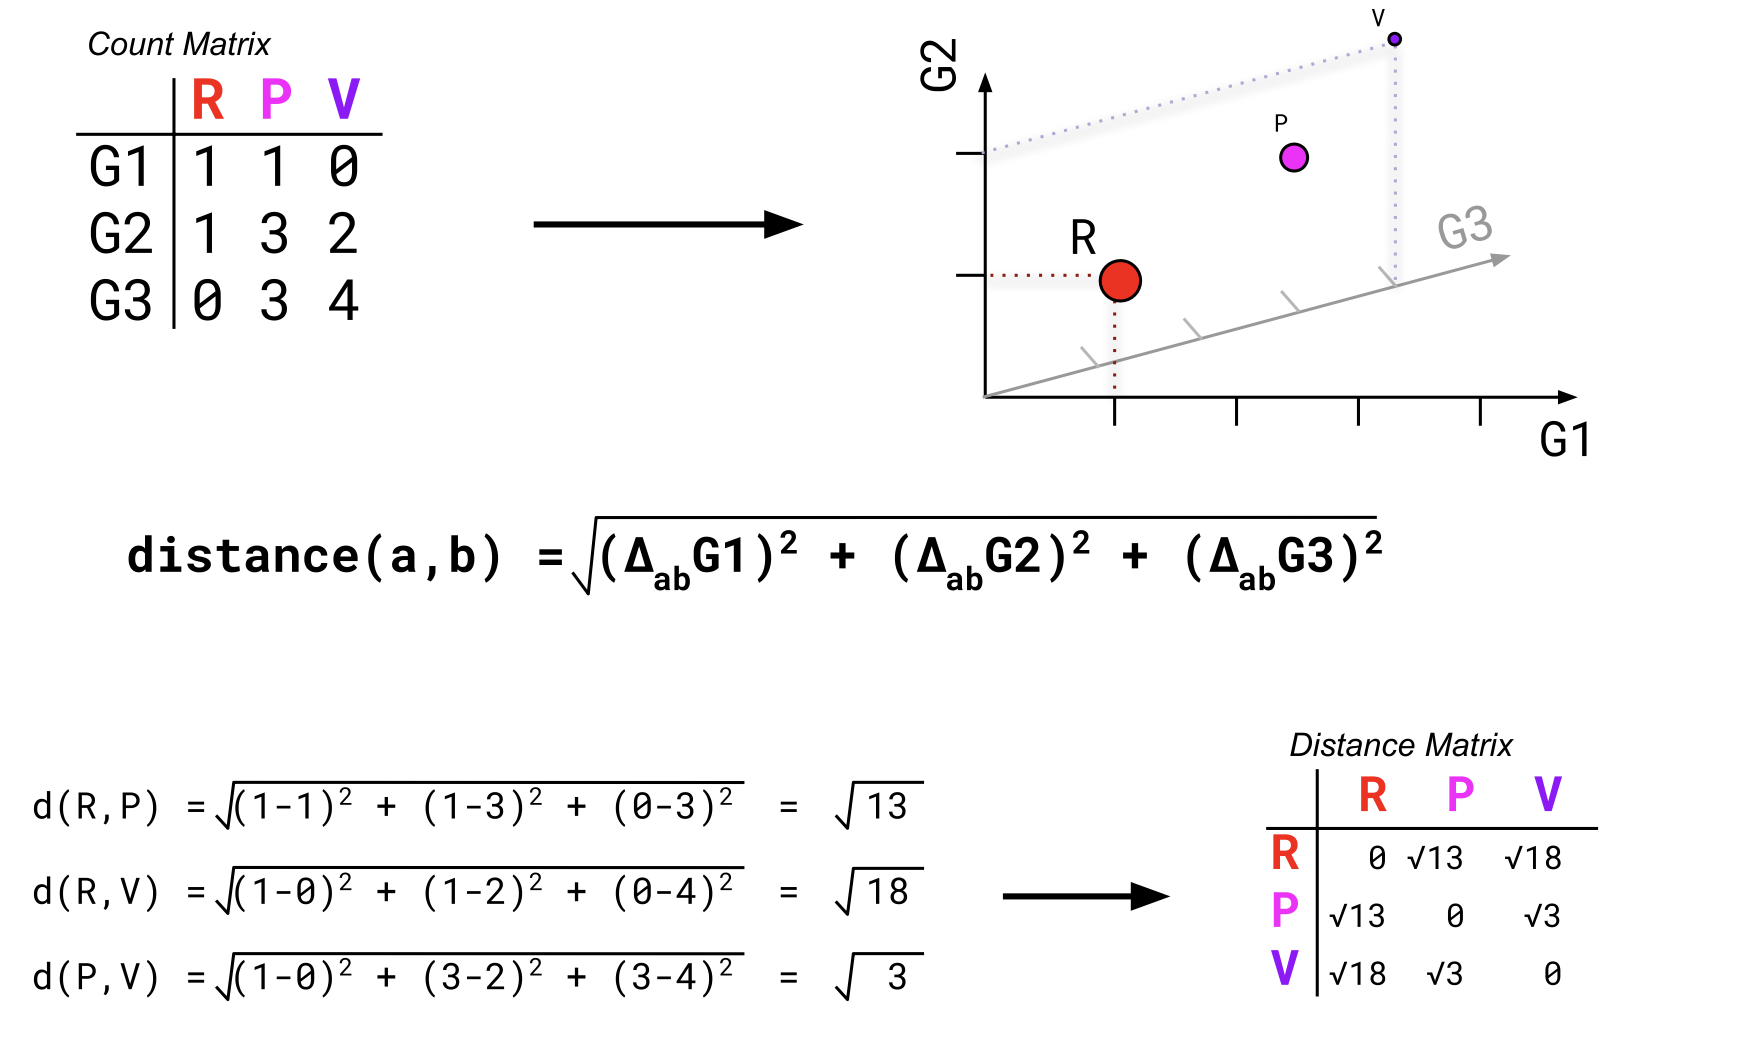
\includegraphics[width=0.5\textwidth]{EuclideanDistance.png}
    \caption{Euclidean Distance for Clustering~\cite{Batut_2018}}
    \label{fig:euclidean_distance}
\end{figure}

It is common to use a simple substitution scheme for nucleic acid sequences.
\begin{figure}[H]
    \centering
    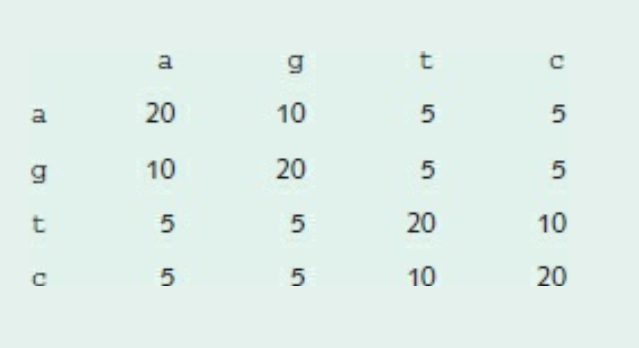
\includegraphics[width=0.5\textwidth]{transitioin .png}
    \caption{Simple transition mutation matrix}
    \label{fig:transition}
\end{figure}
We could also apply the same logic of PAM/BLOSUM to formulate a substitution matrix. 
\begin{figure}[H]
    \centering
    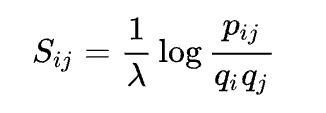
\includegraphics[width=0.5\textwidth]{blosumformula.png}
    \caption{BLOSUM Calculation}
    \label{fig:blosum}
\end{figure}

BLOSUM matrices with higher numbers are used to compare closely related sequences, whereas those with lower numbers are used to compare distantly related sequences~\cite{attwood2003introduction}.

\subsection{Sequence Alignment}
Now that we've discussed how scoring matrices work, we can use them to find optimal alignments.
A well-known algorithms for determining the global best alignments of two sequences is based on a mathematical technique known as dynamic programming.
Both global and local alignment are based on a dynamic programming system.

\begin{enumerate}
    \item Global Alignment - Needleman–Wunsch algorithm
    \item Local Alignment - Smith–Waterman algorithm
\end{enumerate} 

The Needleman-Wunsch algorithm, which is based on dynamic programming, ensures that the optimal alignment of two sequences is found. This algorithm breaks the entire sequence into short sequence segments and uses the solutions of the smaller segments to generate a solution for the entire sequence.
Since the algorithm allows for the detection of gaps, gap penalty is introduced to provide a barrier to arbitrary gap insertion~\cite{lesk_2013_bioinformatics}.

\begin{figure}[H]
    \centering
    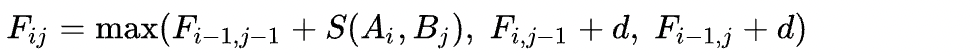
\includegraphics[width=0.5\textwidth]{NW algo.png}
    \caption{Needleman-Wunsch algorithm}
    \label{fig:NW_algo}
\end{figure}

Needleman-Wunsch algorithm starts with 0 at position (2,2)[row,column], filling the scoring for matches and mismatches for the second column and the second row to start with(The first column and row stores the nucleotide/amino acid).
Calculate the score for each cell by going through the cells row by row. The score is calculated by adding the appropriate score for match, mismatch, or gap penalty to the maximum scores of the cells to the left, top, or top-left of the cell.

Smith-Waterman algorithm is applied to find the common regions of similarity. The main differences with the Needleman-Wunsch algorithm is that negative scoring matrix cells are set to zero. 
The traceback method is used after scoring the second column and row as zeros (the nucleotide/amino acid is stored in the first column and row).Traceback based on the source of each score recursively until 0 is encountered, starting with the element with the highest score.

Apply the traceback process starting at the other's highest score outside the trace of the best alignment to obtain other best local alignments~\cite{attwood2003introduction}.

\begin{figure}[H]
    \centering
    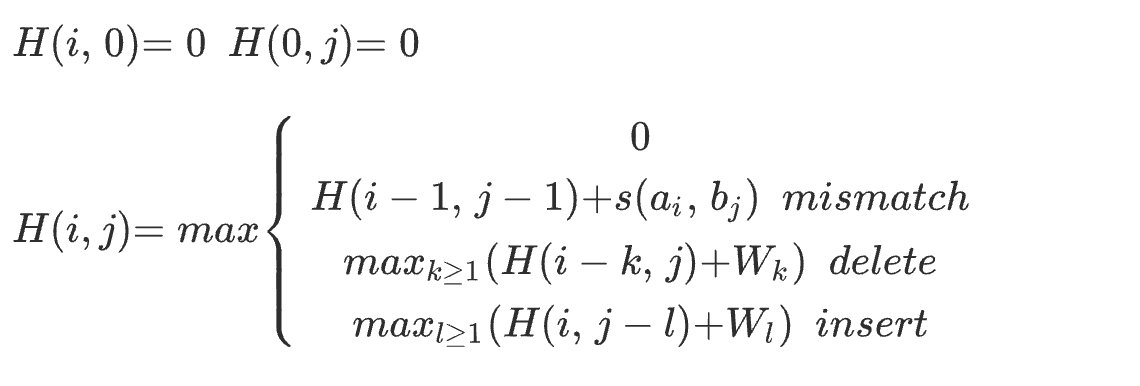
\includegraphics[width=0.5\textwidth]{SW algo.png}
    \caption{Smith-Waterman algorithm}
    \label{fig:SW_algo}
\end{figure}

The major differences between Global and Local Alignments are:
\begin{enumerate}
    \item Backtracking, Global(begins lower right), Local(begins largest value)
    \item Negative scores, Global(allow), Local(zeroed out)
\end{enumerate}

\subsection{Clustering}
The program's aim is to find hidden patterns in unlabeled data. Clustering is one approach to unsupervised learning. The goal of cluster analysis is to divide the observations into clusters so that the pairwise dissimilarities between those assigned to the same cluster are less than those assigned to different clusters. There are various types of methods~\cite{clustering2021Prasad}:\\
1. Partitional Clustering\\
2. Hierarchical Clustering\\
3. Fuzzy Clustering\\
4. Neural Network-based Clustering\\
5. Mixture Model Clustering\\
6. Bi-clustering\\

And some more, below are a few example and simple explanations: K-Means and K-Medoids are examples of partitional clustering algorithms.

K-Means, with a number of cluster centres, the algorithm moves the centres to minimise the total within variance, which can be easily implement and it is relatively efficient, however, the downside is that it could be sensitive to outliers which could be solved. The results of using the K -means clustering algorithms are determined by the number of clusters to be searched and the initial configuration assignment.

On the other hand, Hierarchical Clustering requires the user to specify a measure of dissimilarity(scoring matrix) based on pairwise dissimilarities between the sequences or protein data Strategies for hierarchical clustering consist of 2 main kinds: Agglomerative and Divisive, it is used for transforming a proximity matrix into a nested partition which is presented with dendrogram~\cite{franklin2005elements}.

This program has implemented three types of linkage:\\
1. Complete Linkage\\
\begin{figure}[H]
    \centering
    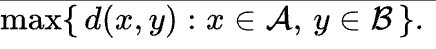
\includegraphics[width=0.5\textwidth]{CompleteLinkage.png}
    \caption{Complete Linkage}
    \label{fig:complete_linkage}
\end{figure}
2. Group Average Linkage\\
\begin{figure}[H]
    \centering
    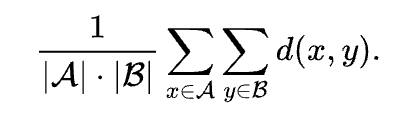
\includegraphics[width=0.5\textwidth]{Aveerage Linkage.png}
    \caption{Group Average Linkage}
    \label{fig:grp_avg_linkage}
\end{figure}
3. Single Linkage
\begin{figure}[H]
    \centering
    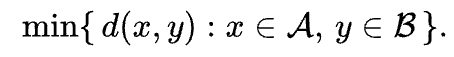
\includegraphics[width=0.5\textwidth]{Single Linkage.png}
    \caption{Single Linkage}
    \label{fig:single_linkage}
\end{figure}

\subsection{Principal component analysis}
Depending on the sample size, a gene expression matrix may be n-dimensional. It could be challenging to visualise data in n-dimensional format with a relatively large data set.

Dimension reduction techniques are required to acquire a set of principal variables and thereby lower the number of random variables.

Using dimension reduction techniques, samples may be described by a few principle variables rather than hundreds of genes. This is quite beneficial for clustering and visualizing the data.

With principle component analysis being one of the most frequent used dimension reduction technique, there are several interpretations of how principle component analysis minimizes the dimension. ~\cite{akalin2020computational}.

The principal component analysis may be performed on the covariance matrix's eigenvectors to determine the directions in which the data have the most variation.
QR decomposition is introduce in order to determinate the eigenvalues and eigenvectors which indicate the direction and the magnitude of variation of the data. 

QR decomposition is a the process of decomposing a matrix X into X = QR where R is a (p + 1) × (p + 1) upper triangular matrix and Q is an N × (p + 1) orthogonal matrix ~\cite{franklin2005elements}.

\begin{figure}[H]
    \centering
    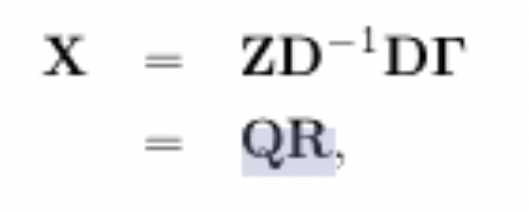
\includegraphics[width=0.5\textwidth]{QR .png}
    \caption{QR decomposition}
    \label{fig:qr_decomposition}
\end{figure}

Dimension reduction is achievable via principal component analysis by ordering the eigenvectors according to their eigenvalues; the greater the eigenvalue, the more variation there is in comparison; this enables the top eigenvector to capture the majority of the data's variance.

\chapter{Software Engineering Method}
With a good understanding of the requirement specification as well as the background theory, this chapter will be focusing on the design process. 

\section{Methodology}
Unlike the waterfall process, which requires a large amount of documentation before any coding can begin.

The Agile approach is a style of project management that divides a project into stages. It necessitates ongoing engagement with stakeholders as well as continual development at each level.
Developers cycle through a process of planning, executing, and assessing once the work starts, enabling them to rework the design and get a better knowledge of the issue along the way.
The agile technique encourages developers to build code as models are created, introducing the concept of test driven development, which ensures that the underlying functionality achieves the desired outcomes.

As the project is designed to be extendable, the agile approach will be preferable to the waterfall since it allows for future user extensions and regular refactoring to maintain the project's long-term sustainability and reliability~\cite{pfleeger2006software}.


\section{Plug-in Architecture}
In general, an application consists of different software units, such as package and library.

The plug-in architecture pattern allows different features to be added into the core application via the plug-ins, providing extensibility as well as feature separation and isolation.

A plug in architecture consists of two types of architecture components: a core system and plug-in modules. 

The core system of a plug-in design pattern often only has the bare minimum of functionality required to keep the system functioning, which means the core system must be aware of which plug-in modules are accessible and how to access them~\cite{richards2015software}.

\subsection{What is plug in}
Plug-ins are software extensions that allow third-party developers to enhance the functionality of software applications and frameworks~\cite{dsouza2012expert}.

Using this project as an example, several additional plug ins have been included inside the clustering package to facilitate functioning, such as the opencsv plug-in for reading CSV files in order to interpret the microarray data (gene expression matrix).

In order for the overall architectural pattern to work, there are several fundamental fundamental principles that must be understood and used. The concept of independently deployed units is the first of these fundamental fundamental notions.

An efficient and simplified delivery pipeline and enhanced scalability are made possible by the plug-in architecture's deployment of each component as a distinct unit, as depicted in the diagram below.

By using the plug-in architecture, users may customise the various types of functionality necessary for their individual requirements by simply adding additional plug-ins to their existing installation. As a result, the package may be tailored to meet the specific requirements of the vast majority of consumers.

\section{UML Package Diagram}
The figure below depicts the package structure in a hierarchical view, which provides a rather more straightforward overview of the package and makes it easier to comprehend.

The UML package diagram displays the relationships between classes and allows us to see the system as a small collection of packages, each of which may be expanded to a larger set of classes~\cite{pfleeger2006software}.

\begin{figure}[H]
    \centering
    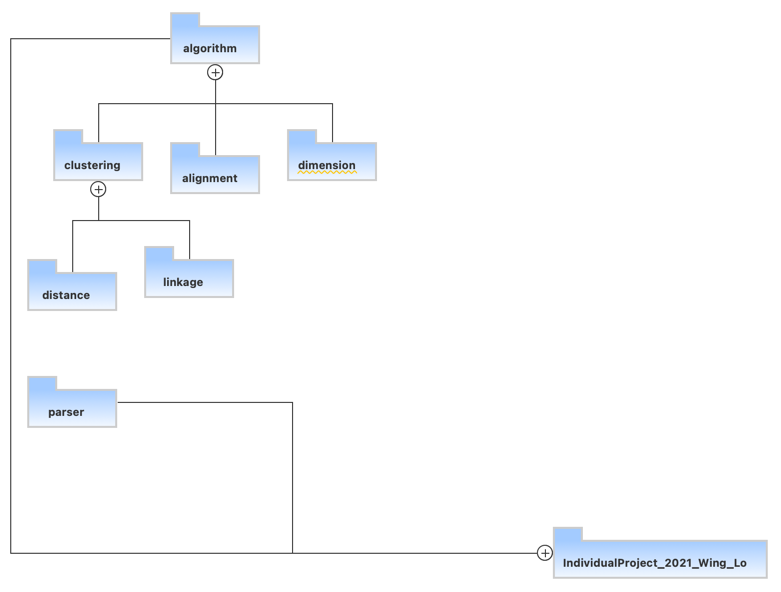
\includegraphics[width=1\textwidth]{packages.umlcd.png}
    \label{fig:package}
\end{figure}

\section{UML Class Diagram}
The UML class diagram below demonstrates the classes, attributes, operations, and their relationships to one another to provide an overview of a software system. The diagram depicts the many categories of items in the system as well as the various sorts of connections between them. It provides a high-level overview of a program~\cite{pfleeger2006software}.

\begin{figure}[H]
    \centering
    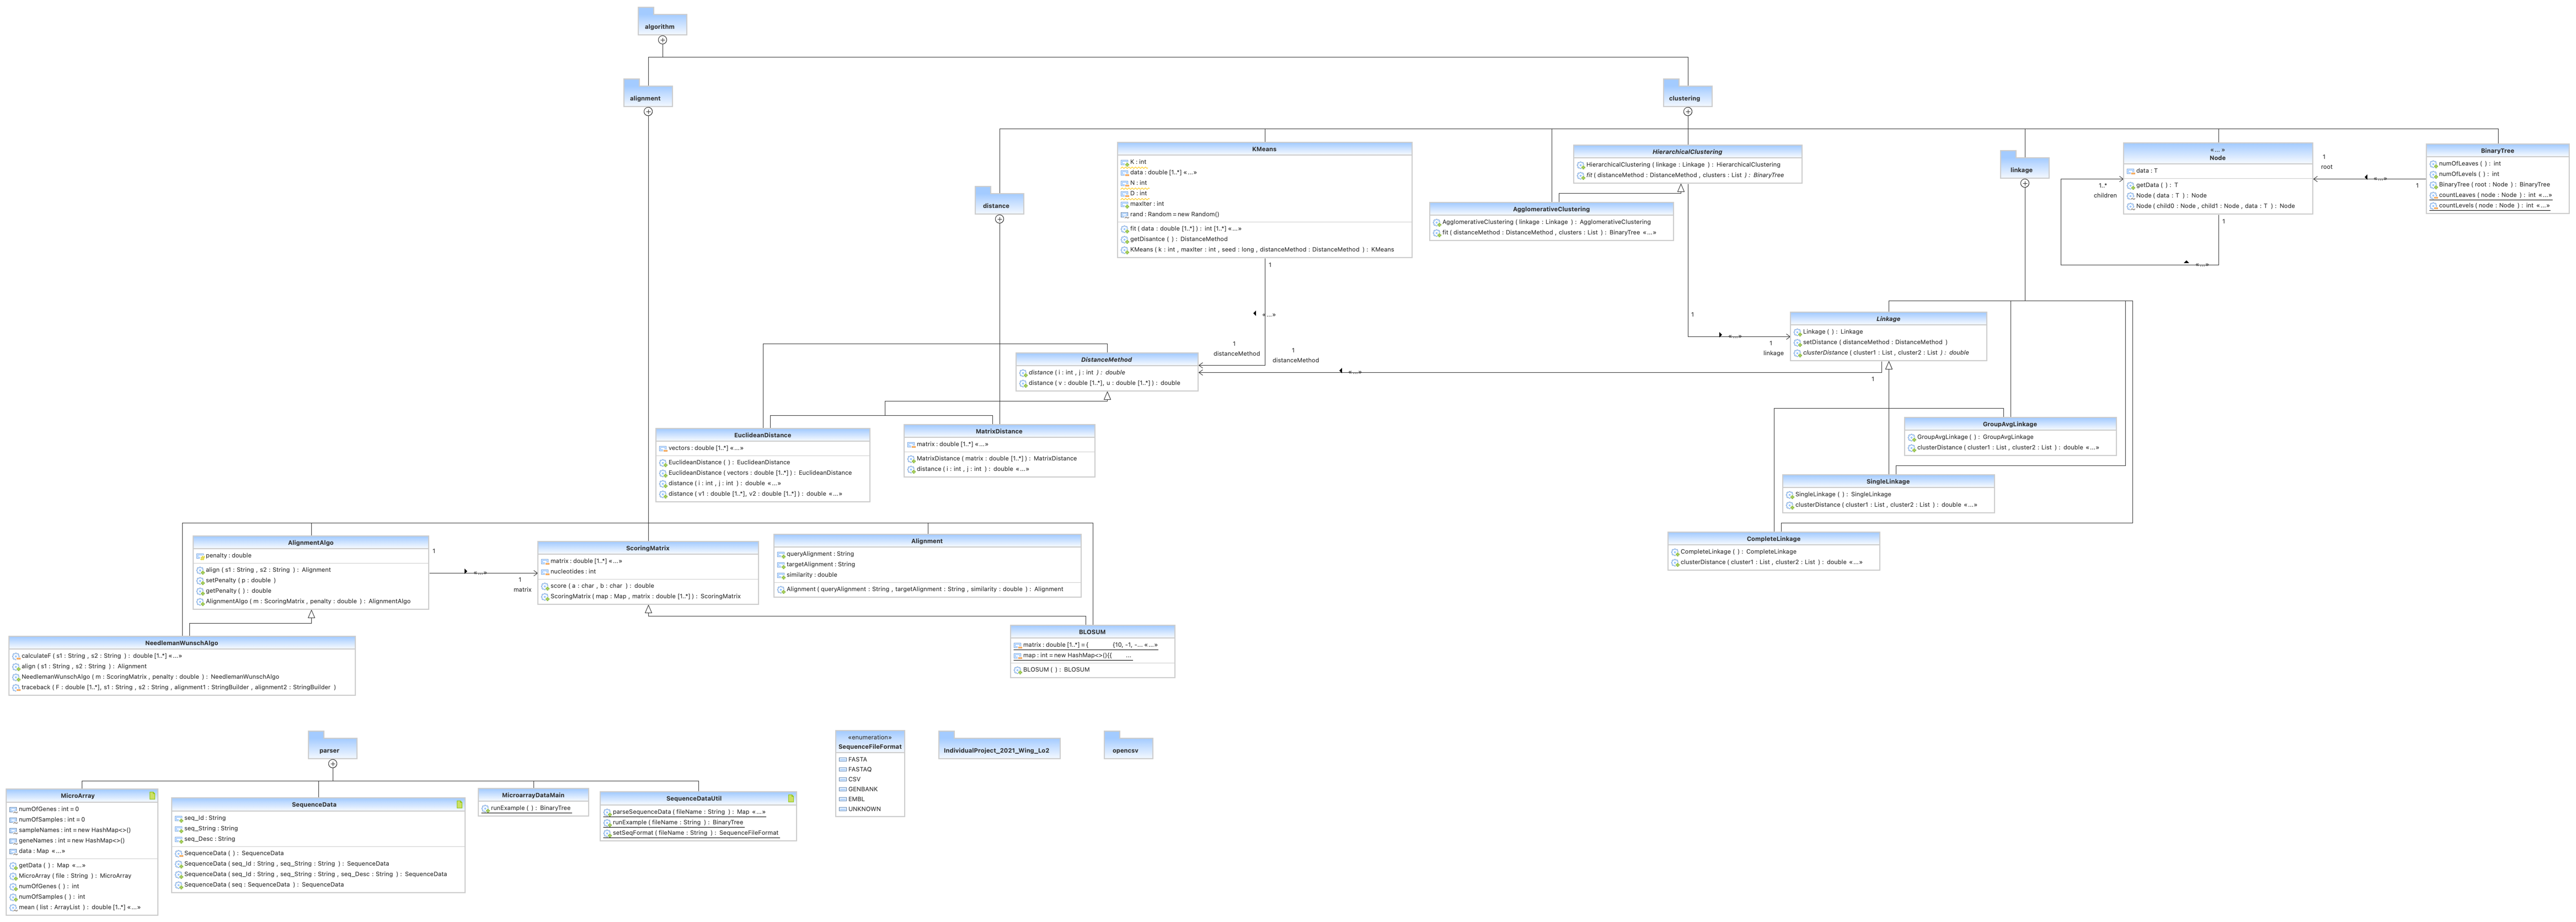
\includegraphics[width=1\textwidth]{IndividualProject_2021_Wing.Lo2.umlcd.png}
    \caption{UML class diagram}
    \label{fig:class_diagram}
\end{figure}

\section{Design Pattern}
The façade software structure design pattern, as well as the strategy behavioural software design pattern, will be used in the development of the package.

When dealing with a complicated subsystem, the facade design makes it simpler to use by creating a facade class that offers a single, more acceptable interface, thereby simplifying its usage and decreasing its complexity~\cite{freeman2020head}.

It is possible to change out algorithms using the Strategy Pattern, which includes a family of algorithms. The algorithm's technique permits it to adapt without being influenced by the users who make use of the algorithm~\cite{freeman2020head}.

As an example, the hierarchical clustering package may be used to construct multiple hierarchical clustering algorithms, one of which is agglomerative clustering. By extending the class, the user may build any other form of hierarchical clustering algorithm without having to write directly into the hierarchical class. This decreases the likelihood of any current codes being broken.The hierarchical class may also be used with just one line of code with different linkage options.

\begin{verbatim}
    HierarchicalClustering clustering = new AgglomerativeClustering(new SingleLinkage())
\end{verbatim}

\begin{figure}[H]
    \centering
    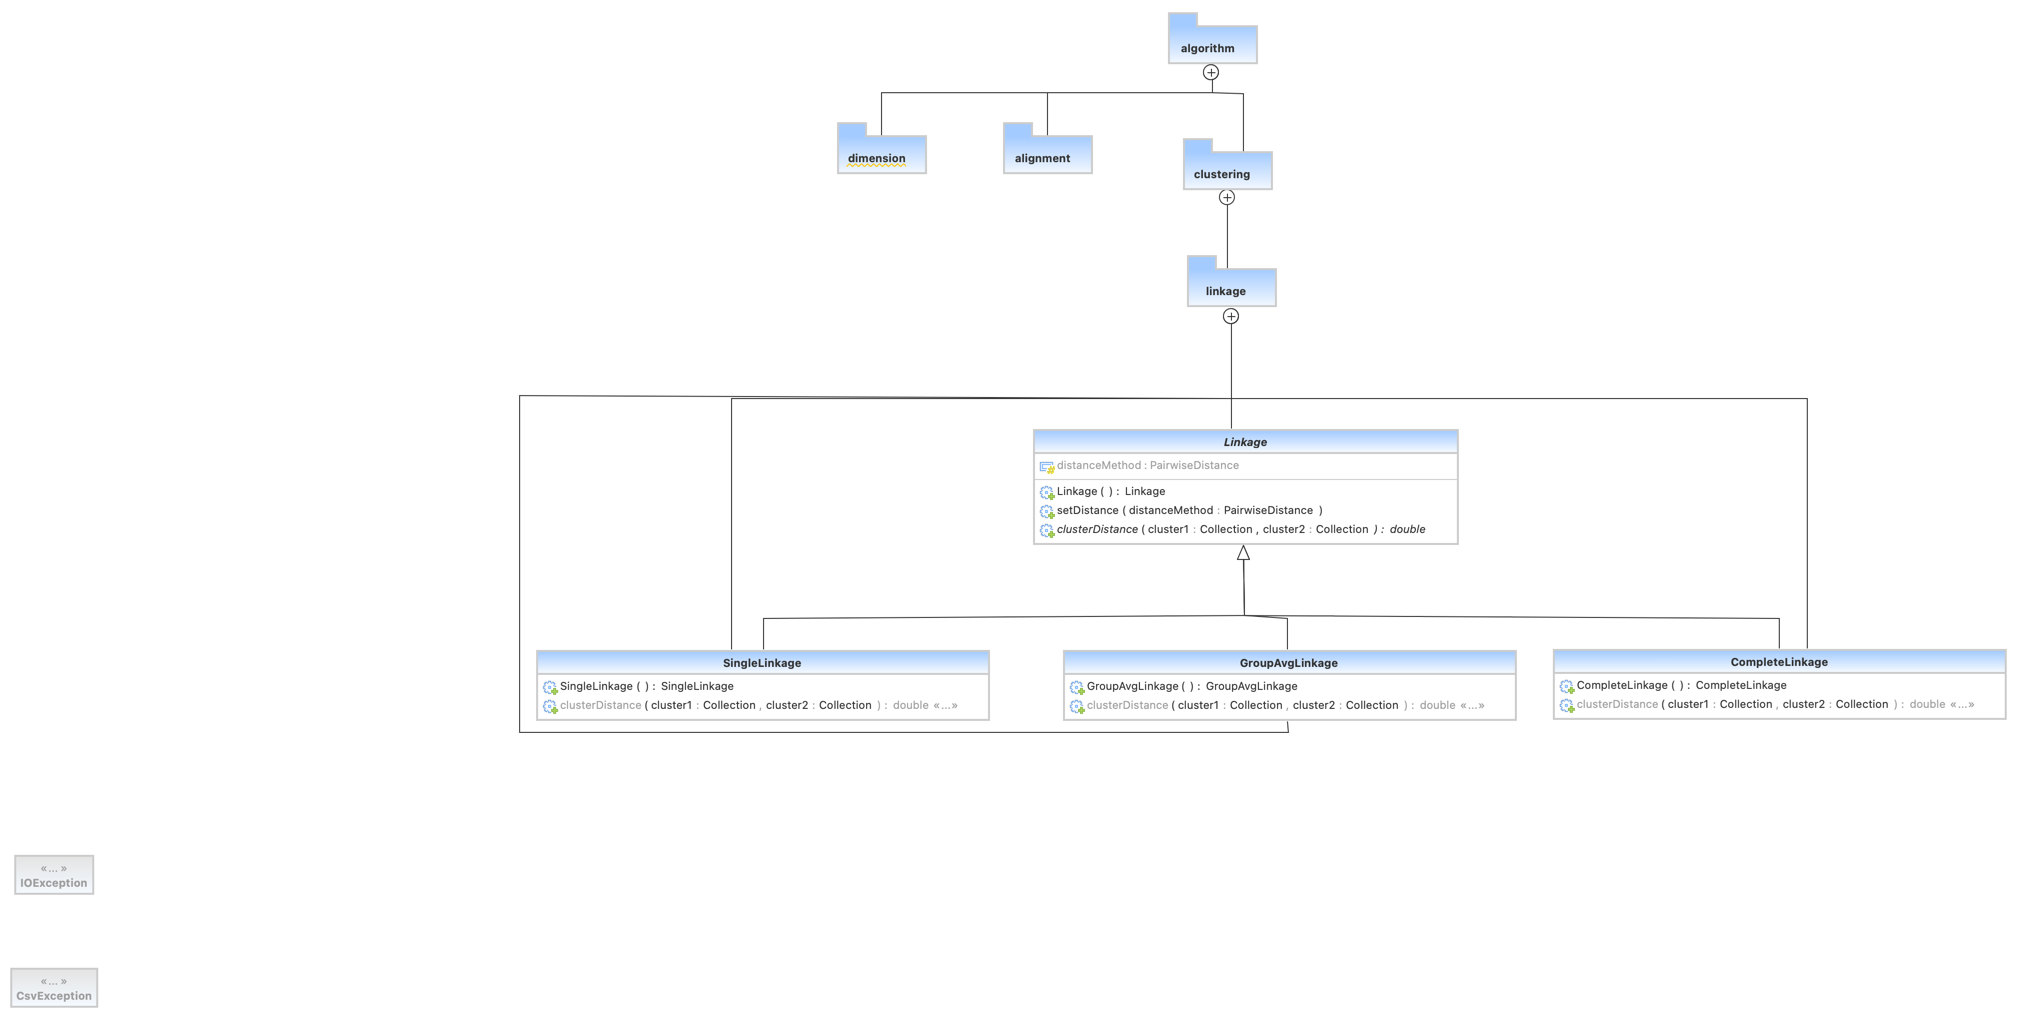
\includegraphics[width=1\textwidth]{linkage.umlcd.png}
    \caption{clustering}
    \label{fig:linkage_class_diagram}
\end{figure}
\section{Testing}
Testing is a critical component of framework implementation. The application's components will be employed in a wide variety of circumstances and must therefore be very trustworthy. To assure this reliability, the application was subjected to various stages of testing~\cite{gewehr2007bioweka}.

In this project, unit testing were used to test out the parser, alignment, clustering and visualisation functions. 
\subsection{JUnit testing}
JUnit is an open-source framework for unit testing the Java . It includes test cases that must be re-run whenever new code is introduced. This is done to ensure that there are no errors in the code.

JUnit has a number of graphs that illustrate the progress of a test. When the test goes smoothly, the graph exhibits a green colour; when the test fails, the graph displays a red hue. JUnit Testing helps developers to write code that is extremely dependable and error-free ~\cite{appel2015testing}.

\chapter{Implementation}
This package was created as a foundation on which bespoke solutions might be built, rather than as a particular solution to a specific problem. As a result, specific framework building criteria must be followed~\cite{gewehr2007bioweka}.

Reusable, extendable, and maintainable frameworks are desirable. An extensible application is one that can be readily extended without altering its original code base, allowing additional plug-ins or modules to improve its capabilities.~\cite{freeman2020head}.

\section{Extendibility}
Extendibility is a measure of a system's ability to be extended and the amount of work necessary to do so. The addition of new functionality or the change of existing functionality are both examples of extensions. The idea allows for improvements without compromising the system's present functionalities~\cite{gewehr2007bioweka}.
This is achievable because to object oriental programming languages' inheritance and confinement properties.

Extendibility relies on the interface. For example, the class NeedlemanWunschAlgo extends AlignmentAlgo, n alignment method is represented by a component that implements the alignment interface.
NeedlemanWunschAlgo component holds references to two other components: a ScoringMatrix and an Alignment component.

\section{Reusability}
Reuse necessitates evaluating goods from present and future development initiatives to see whether the kind and quality are appropriate. One of the primary promises offered by object oriented programming languages is code reuse, and inheritance is the technique used to make this promise a reality~\cite{pfleeger2006software}.

In Java, inheritance is accomplished via the use of extensions.
\begin{verbatim}
public class AlignmentAlgo {...}

public class NeedlemanWunschAlgo extends AlignmentAlgo {...}
\end{verbatim}

\section{Proof of concept}
The program will be written in Java languages as required. Following the requirement of the project is to be extensible in different ways, which means Java plug-ins will be needed. We will be also be using strategy structure. 

This first step will be implementing a component that is able to read the data from different types of database.

For the beginning database, two of the most common used file types will be chosen, CSV and FASTA, this should display the data separate on each line, so it can be used for, clustering.

Further there should be a function that makes it possible to read which input file is used. Importing opencsv allows the program to read csv file format, below are the proof of concept codes for both FASTA parser for sequence data type and the CSVparser for microarray data type.

\label{FASTAparser}
\begin{verbatim} 
import java.util.*;
import java.io.*;

public static Map<String, String> parseSequenceData(String fileName) throws IOException{
        BufferedReader br = new BufferedReader(new FileReader(fileName));

        String line;
        String seq_id = null;
        Map<String, String> seqMap = new LinkedHashMap<>();

        while((line = br.readLine()) != null){
            line = line.trim();
            if(line.startsWith(">")){
                seq_id = line.substring(1);
            } else{
                seqMap.put(seq_id, line);
                new SequenceData(seq_id, line);
            }
        }
        return seqMap;
    }

\end{verbatim}

\begin{verbatim}
import java.io.FileReader;
import java.io.IOException;
import java.util.*;

import com.opencsv.CSVReader;
import com.opencsv.exceptions.CsvException;
public class MicroArray {
    int numOfGenes = 0;
    int numOfSamples = 0;
    Map<String, Integer> sampleNames = new HashMap<>();
    Map<String, Integer> geneNames = new HashMap<>();
    Map<String, double[]> data;

    double[] mean(ArrayList<double[]> list) {
        int n = list.get(0).length;
        int m = list.size();
        double[] result = new double[n];

        for (int i = 0; i < list.size(); ++i) {
            for (int j = 0; j < n; ++j) {
                result[j] += list.get(i)[j] / m;
            }
        }

        return result;
    }

    public MicroArray(String file) throws IOException, CsvException {
        CSVReader reader = new CSVReader(new FileReader(file));
        List<String[]> myEntries = reader.readAll();
        numOfGenes = myEntries.size() - 1;
        numOfSamples = myEntries.get(0).length - 1;
        Map<String, ArrayList<double[]>> temp = new HashMap<>();
        data = new HashMap<>();

        for (int j = 0; j < numOfSamples; ++j) {
            sampleNames.put(myEntries.get(0)[j + 1], j);
        }

        for (int i = 0; i < numOfGenes; ++i) {
            String[] row =  myEntries.get(i + 1);
            String geneName = row[0];
            double[] d = new double[numOfSamples];
            for (int j = 0; j < numOfSamples; ++j) {
                d[j] = Double.parseDouble(row[j + 1]);
            }

            if (geneNames.containsKey(geneName)) {
                temp.get(geneName).add(d);
            }
            else {
                ArrayList<double[]> list = new ArrayList<>();
                list.add(d);
                temp.put(geneName, list);
            }
            geneNames.put(geneName, i);
        }
        for (Map.Entry<String, ArrayList<double[]>> pair : temp.entrySet()) {
            String geneName = pair.getKey();
            ArrayList<double[]> array = pair.getValue();
            if (array.size() > 1) {
                data.put(geneName, mean(array));
            } else {
                data.put(geneName, array.get(0));
            }
        }
    }

\end{verbatim}

Sequence alignment methods are required prior to clustering in order to detect similarities between data. The diagram \ref{fig:process} below depicts how the program works with various data file formats and the corresponding alignment method.
\begin{figure}[H]
\centering
     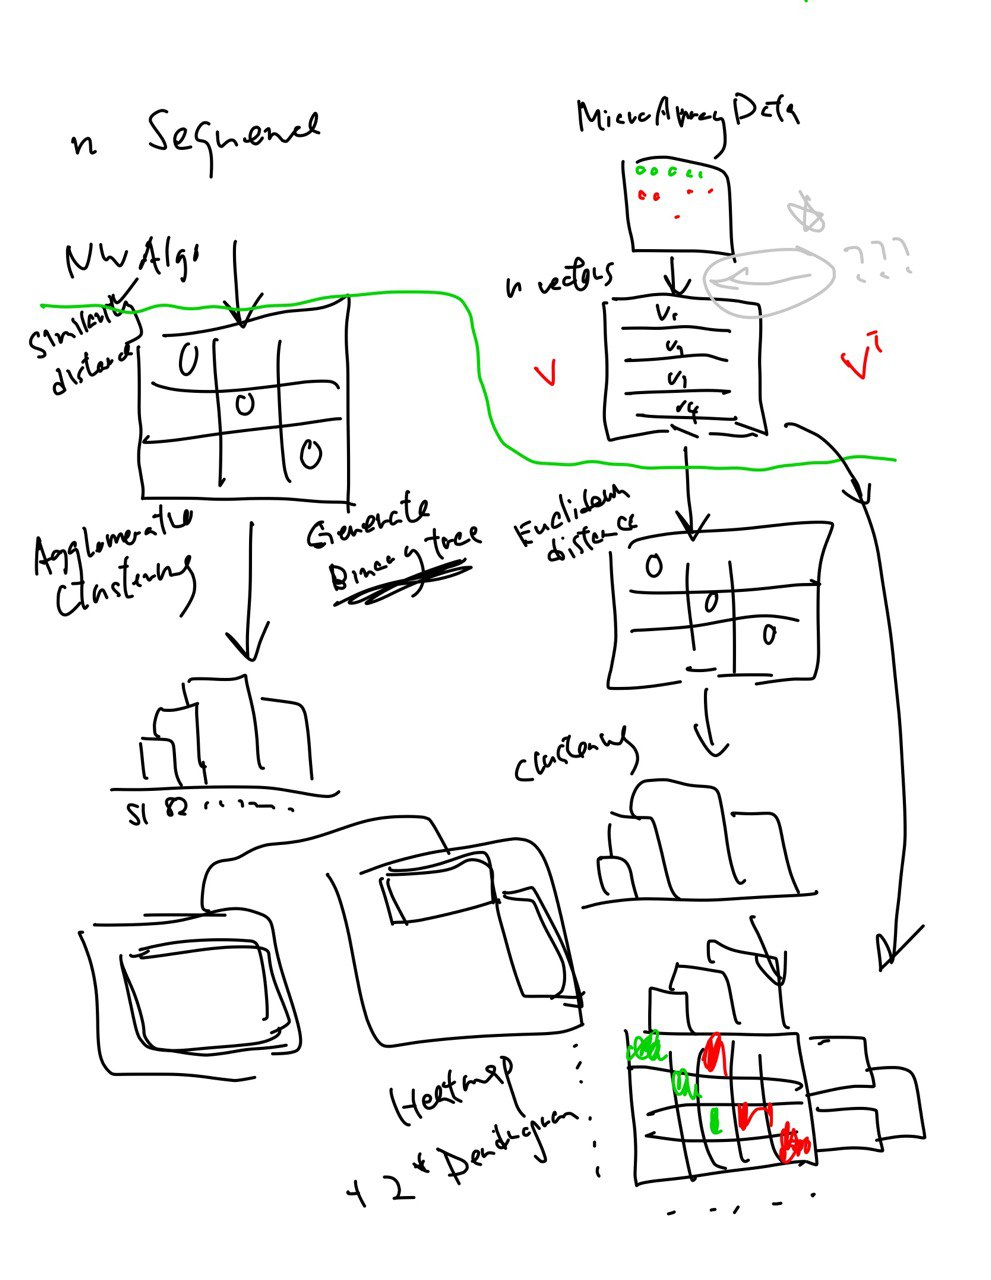
\includegraphics[width=0.5\textwidth]{process.JPG}
      \caption{Process for various data format }
       \label{fig:process}
\end{figure}

The coding below depicts the created similarity distance matrix, which will be the BLOSUM matrix as a final deliverable.
\begin{verbatim}
import java.util.HashMap;
import java.util.Map;

public class BLOSUM extends ScoringMatrix {
    private static final double[][] matrix = {
            {10, -1, -3, -4},
            {-1, 7, -5, -3},
            {-3, -5, 9 , 0},
            {-4, -3, 0 , 8},
    };
    private static final Map<Character, Integer> map = new HashMap<>(){{
        put('A', 0);
        put('G', 1);
        put('C', 2);
        put('T', 3);
    }};
    public BLOSUM() {
        super(map, matrix);
    }
}
\end{verbatim}

Different parsers provide different results; for k means clustering, the microarray data needs principal component analysis to reduce the n-dimensional array to a two-dimensional array.

When it comes to hierarchical clustering, the gene expression data will need to be aligned pairwise before a dendrogram can be generated.

When it comes to clustering methods, agglomerative clustering is used to analyse the data as the first step.

\begin{verbatim}
import algorithm.clustering.distance.Distance;
import algorithm.clustering.linkage.Linkage;

import java.util.ArrayList;
import java.util.List;

public class AgglomerativeClustering extends HierarchicalClustering {

    public AgglomerativeClustering(Linkage linkage){
        super(linkage);
    }

    @Override
    public BinaryTree fit(Distance distance, List<List<Integer>> clusters) {
        this.linkage.setDistance(distance);
        List<Node> nodes = new ArrayList<>();
        // {{1}. {2}, ....}
        for (List<Integer> c : clusters) {
            nodes.add(new Node(c.get(0)));
        }
        while (clusters.size() > 1) {
            int index_i = 0;
            int index_j = 0;
            double minimum = Double.MAX_VALUE;
            for (int i = 0; i < clusters.size(); ++i) {
                for (int j = i + 1; j < clusters.size(); ++j) {
                    // a defined distance measurement for two clusters - linkage method
                    // distance between two clusters
                    // a kind of aggregation
                    double d = this.linkage.clusterDistance(clusters.get(i), clusters.get(j));
                    if (d < minimum) {
                        minimum = d;
                        index_i = i;
                        index_j = j;
                    }
                }
            }

            Node left = nodes.get(index_i);
            Node right = nodes.get(index_j);
            nodes.set(index_i, new Node(left, right, minimum));
            nodes.remove(index_j);

            List<Integer> c_i = clusters.get(index_i);
            List<Integer> c_j = clusters.get(index_j);
            c_i.addAll(c_j);
            clusters.remove(index_j);
        }
        Node root = nodes.get(0);
        BinaryTree tree = new BinaryTree(root);
        return tree;
    }
}
\end{verbatim}

The other clustering method avaliable will be the K means clustering.

\begin{verbatim}
    package algorithm.clustering;

import algorithm.clustering.distance.DistanceMethod;
import org.apache.commons.lang3.tuple.ImmutablePair;
import org.apache.commons.lang3.tuple.Pair;

import java.util.Arrays;
import java.util.Random;

public class KMeans {

    private int k;

    private int maxIteration;

    private DistanceMethod distanceMethod;
    private int seed;

    private String initialMethoid;

    public class KMeansResult {
        public int[] labels;
        public double[][] centroids;
        public double inertia;

        public KMeansResult(int[] labels, double[][] centroids, double inertia) {
            this.labels = labels;
            this.inertia = inertia;
            this.centroids = centroids;
        }

    }

    public KMeans(int k, int maxIteration, DistanceMethod distanceMethod, int seed, String initialMethoid) {
        this.k = k;
        this.maxIteration = maxIteration;
        this.distanceMethod = distanceMethod;
        this.seed = seed;
        // kmeans++ or random
        this.initialMethoid = initialMethoid;
    }

    private double[][] randomCentroids(double[][] data, int k) {
        int d = data[0].length;
        double[] mins = new double[d];
        double[] maxs = new double[d];
        Arrays.fill(mins, Double.POSITIVE_INFINITY);
        Arrays.fill(maxs, Double.NEGATIVE_INFINITY);

        for (double[] record : data) {
            for (int i = 0; i < d; ++i) {
                mins[i] = Math.min(mins[i], record[i]);
                maxs[i] = Math.max(maxs[i], record[i]);
            }
        }

        Random rand = new Random(seed);

        double[][] centroids = new double[k][d];
        for (int i = 0; i < k; i++) {
            for (int j = 0; j < d; ++j) {
                centroids[i][j] = rand.nextDouble() * (maxs[j] - mins[j]) + mins[j];
            }
        }
        return centroids;
    }

    private double[][] KmeansPlusPlus(double[][] data, int k) {
        int d = data[0].length;
        int n = data.length;
        double[][] centroids = new double[k][d];
        double[] distToClosestCentroid = new double[n];
        double[] weightedDistribution  = new double[n];

        Random gen = new Random(seed);
        int choose = 0;

        for (int c = 0; c < k; c++) {
            if (c == 0)
                choose = gen.nextInt(n);
            else {
                for (int p = 0; p < n; p++) {
                    double tempDistance = distanceMethod.distance(data[p], centroids[c - 1]);

                    if (c == 1)
                        distToClosestCentroid[p] = tempDistance;

                    else {
                        if (tempDistance < distToClosestCentroid[p])
                            distToClosestCentroid[p] = tempDistance;
                    }

                    if (p == 0)
                        weightedDistribution[0] = distToClosestCentroid[0];
                    else
                        weightedDistribution[p] = weightedDistribution[p - 1] + distToClosestCentroid[p];

                }

                double rand = gen.nextDouble();
                for (int j = n - 1; j > 0; j--) {
                    if (rand > weightedDistribution[j - 1] / weightedDistribution[n - 1]) {
                        choose = j;
                        break;
                    }
                    else
                        choose = 0;
                }
            }

            System.arraycopy(data[choose], 0, centroids[c], 0, d);
        }
        return centroids;
    }

    private Pair<Integer, Double> nearestCentroid(double[][] centroids, double[] record) {
        double minDistance = Double.POSITIVE_INFINITY;
        int k = -1;
        for (int i = 0; i < centroids.length; ++i) {
            double dist = distanceMethod.distance(record, centroids[i]);
            if (dist < minDistance) {
                minDistance = dist;
                k = i;
            }
        }
        return new ImmutablePair<>(k, minDistance);
    }

    public KMeansResult fit(double[][] data) {
        int n = data.length;
        int d = data[0].length;

        double[][] centroids = (this.initialMethoid.equals("kmeans++"))? KmeansPlusPlus(data, k) : randomCentroids(data, k);

        int[] labels = new int[n];
        double inertia = 0;

        for (int iter = 0; iter < maxIteration; iter++) {
            inertia = 0;
            for (int i = 0; i < n; i++) {
                Pair<Integer, Double> pair = nearestCentroid(centroids, data[i]);
                int index = pair.getLeft();
                double minDist = pair.getRight();
                inertia += minDist * minDist;
                labels[i] = index;
            }

            int[] count = new int[k];
            // initialize centroid
            for (int i = 0; i < k; i++) {
                Arrays.fill(centroids[i], 0);
            }
            // relocate centroid
            for (int i = 0; i < n; i++) {
                int cluster = labels[i];
                for (int j = 0; j < d; j++) {
                    centroids[cluster][j] += data[cluster][j];
                }
                count[cluster] += 1;
            }

            for (int i = 0; i < k; i++) {
                for (int j = 0; j < d; j++) {
                    centroids[i][j] /= count[i];
                }
            }

            if (iter == maxIteration - 1) {
                break;
            }
        }
        return new KMeansResult(labels, centroids, inertia);
    }

    public int getK() {
        return k;
    }

    public void setK(int k) {
        this.k = k;
    }

    public int getMaxIteration() {
        return maxIteration;
    }

    public void setMaxIteration(int maxIteration) {
        this.maxIteration = maxIteration;
    }


    public void setDistanceMethod(DistanceMethod distanceMethod) {
        this.distanceMethod = distanceMethod;
    }
}
\end{verbatim}

Then, the implementation of the visualising the data that is produced from the algorithm, which we will use open source plugins libraries, we will be visualising the data using dendrogram~\cite{Macdonald2011Analysis} shown in Fig.~\ref{fig:ex_dendrogram} and scatter plot in Fig.~\ref{fig:ex_heatmap+dendrogram} as a draft of concept.

\begin{figure}[H]
\centering
     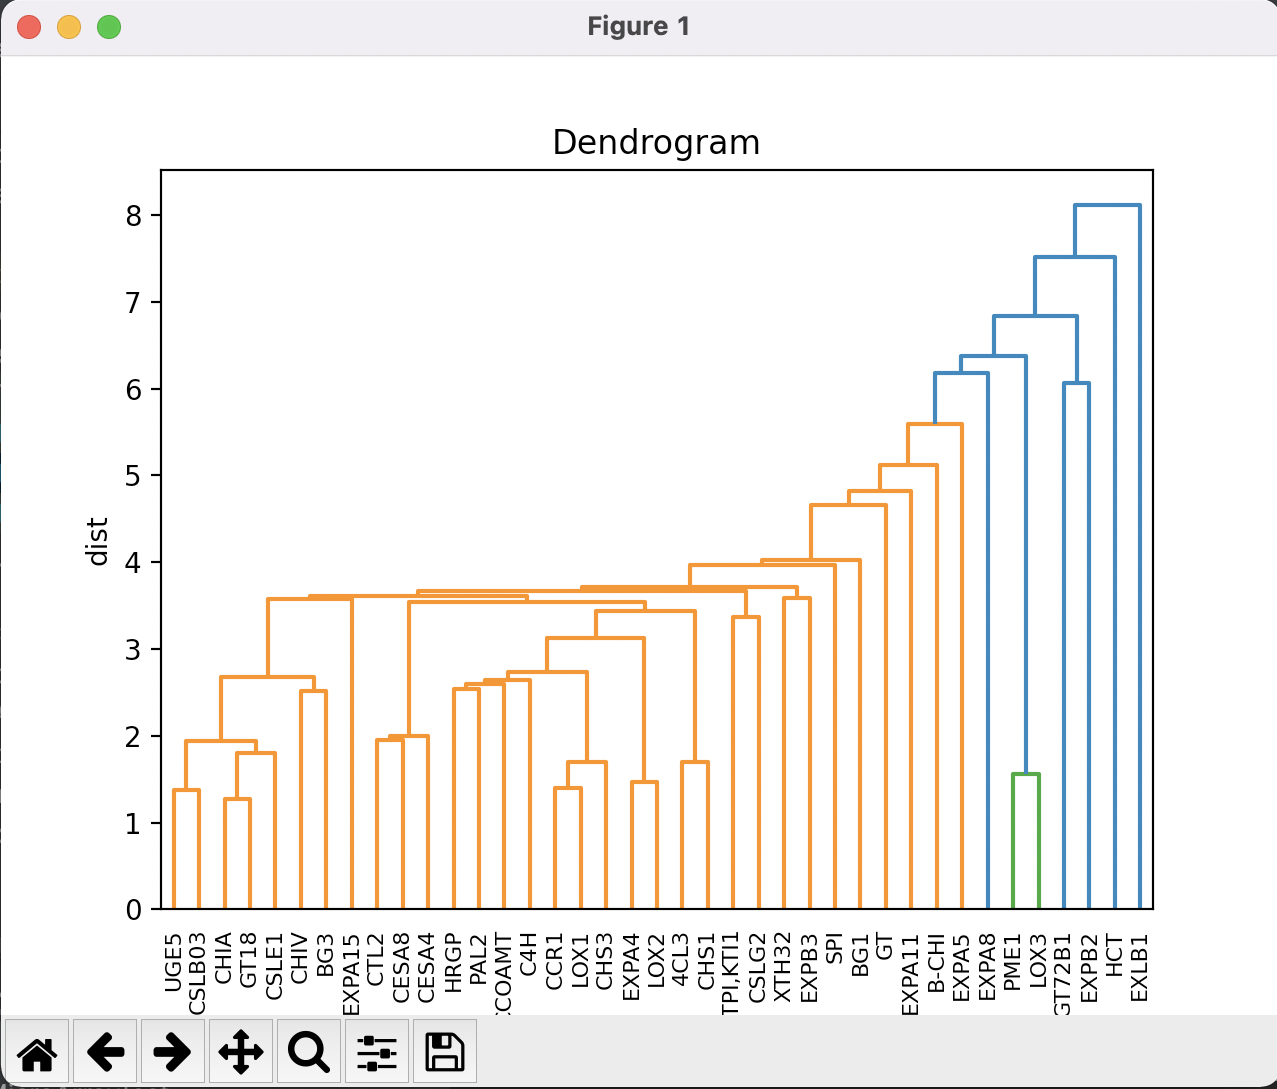
\includegraphics[width=0.5\textwidth]{Rplot02.png}
      \caption{Example: Dendrogram for gene expression matrix }
       \label{fig:ex_dendrogram}
\end{figure}


\begin{figure}[H]
\centering
     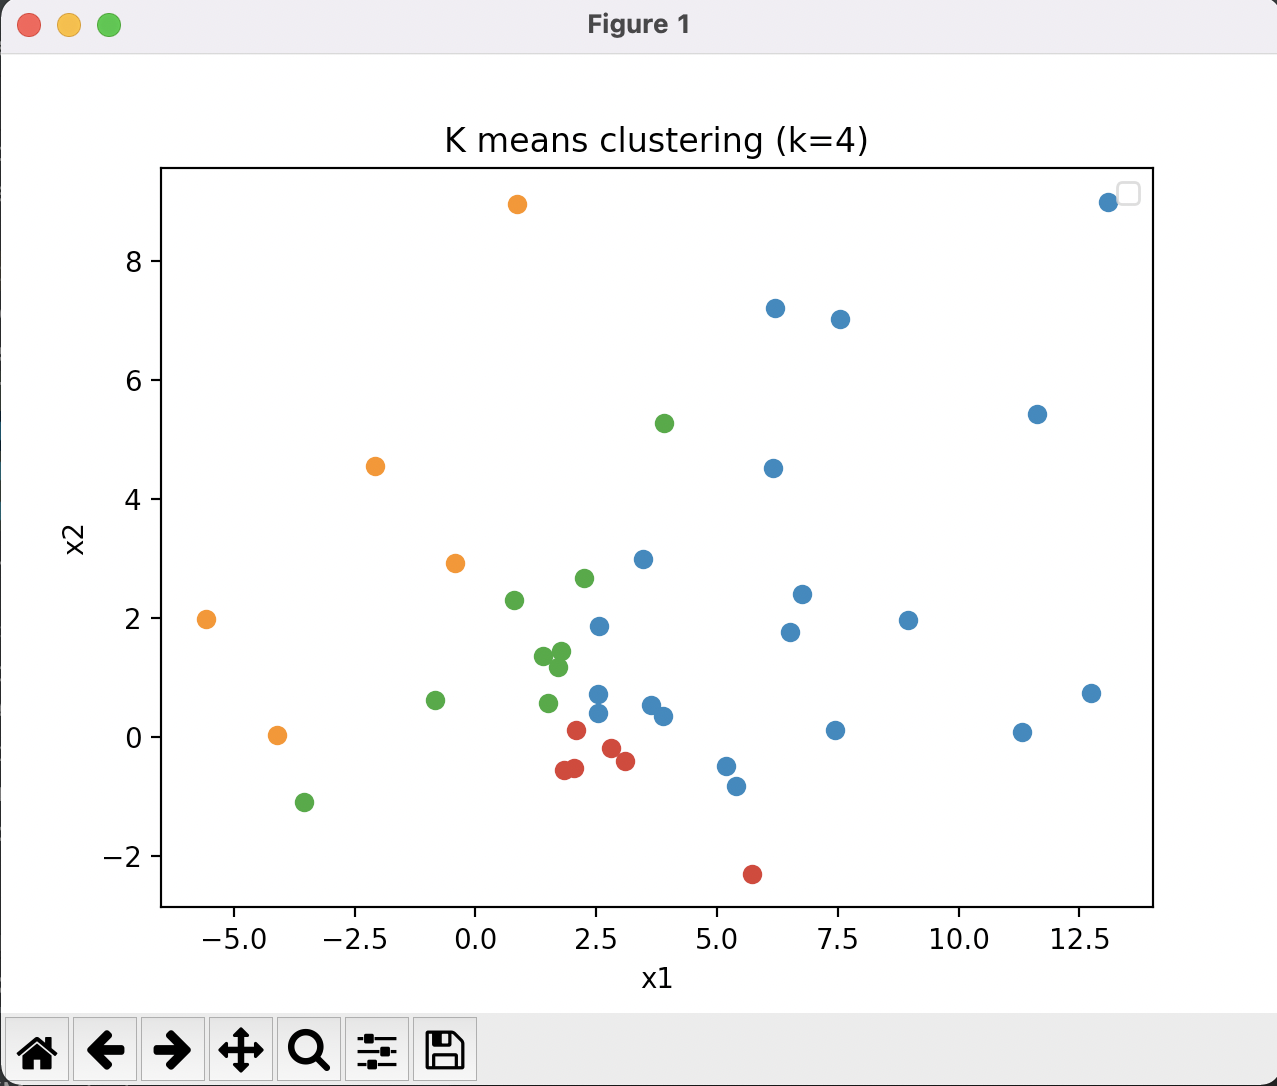
\includegraphics[width=0.5\textwidth]{Scatter Plot.png}
      \caption{Example: Scatter plot with k means clustering}
       \label{fig:scatter_plot}
\end{figure}

As stated in Section \ref{1.2}, the following proof of concept demonstrates the further extension idea of translating a DNA sequence using the standard genetic code~\cite{lesk2019introduction}~\cite{bal2007java}.


\begin{verbatim} 
import table.standardGeneticCode;
import parser.sequence;
import map.DNA, map.RNA, map.AA;
public static int getSequenceType(String sequence) throws IOException{
    Sequence sq = new Sequence(filename);
    String[] strings = sq.split(sq);
    int numbOfAA = 0; 
    
    for (int i = 0; i < strings.length; i++) { 
    numbOfAA += strings[i].length(); 
    }
    int length = sq.length();
    int numbOfRNA = lenght - numbOfAA;
    
    strings = sq.split(sequence);
    int numbOfDNA = 0;
    for (int i = 0; i < strings.length; i++) { 
    numbOfDNA += strings[i].length();
    }
    int numbOfUs = length -  numbOfDNA;
    if (numbOfDNA / (double)length > 0.85){
    return TYPE_DNA;
    }else if ((numbOfDNA + numbOfUs) / (double)length > 0.85) {
        return TYPE_RNA;
    } else {
        return TYPE_PROTEIN;
    }
}
} 
\end{verbatim}

\section{Packages}
A package is a namespace that contains a collection of related classes and interfaces. As Java software might have hundreds or thousands of individual classes, it makes sense to keep things organised by grouping similar classes and interfaces into packages.

This section will show the user how to extend to this package.
\subsection{parsers}
The parser package aims to parse biological data, input of both the sequence and microarray data will output n dimensional array.

The parser package parses two distinct types of data files and formats.

The FASTA file format is used to store sequence data, whereas the CSV file format is used to store gene expression matrix data (microarray data).

If a programmer wishes to expand the package with other parsers, they may simply add them to the parser package.
\subsection{algorithm}
The algorithm package consists of three other packages such as alignment, clustering and dimension.
\subsection{alignment}
As for the alignment package, if developer would like to add an additional alignment algorithm such as the local alignment method, this can be easily done by extending to the Alignment Algo class.
\begin{verbatim}
public class NeedlemanWunschAlgo extends AlignmentAlgo
\end{verbatim}
If developer wish to add an additional scoring matrix it can also be done by extending to the scoring matrix class.
\begin{verbatim}
public class BLOSUM extends ScoringMatrix 
\end{verbatim}
\subsection{clustering}
There are two packages located inside of the clustering package, one of which is the linkage package and the other is the distance package.

Inside of the distance package, with distance method being the interface and the pairwise distance being the abstract class, if the developer wish to add different distance matrix for clustering, simply extend to the pairwise distance class and implement to the distance matrix interface.

\begin{verbatim}
public class EuclideanDistance extends PairwiseDistance implements DistanceMethod {
    private double[][] vectors;

    public EuclideanDistance() {
    }

    public EuclideanDistance(double[][] vectors) {
        this.vectors = vectors;
    }

    @Override
    public int size() {
        return vectors.length;
    }

    @Override
    public double distance(int i, int j) {
        return distance(vectors[i], vectors[j]);
    }

    @Override
    public double distance(double[] v1, double[] v2) {
        double sum = 0;
        for (int d = 0; d < v1.length; ++d) {
            sum += Math.pow(v1[d] - v2[d], 2);
        }
        return Math.sqrt(sum);
    }
}
\end{verbatim}

Inside of the linkage package, there is a linkage interface, if the developer wish to add another linkage method, simply extends to the linkage interface.

\begin{verbatim}
import java.util.Collection;

public class SingleLinkage extends Linkage {
    public SingleLinkage(){
        super();
    }

    @Override
    public double clusterDistance(Collection<Integer> cluster1, Collection<Integer> cluster2) {
        double shortest = Double.MAX_VALUE;
        for (int u : cluster1) {
            for (int v: cluster2) {
                shortest = Math.min(shortest, this.distanceMethod.distance(u, v));
            }
        }
        return shortest;
    }
}
\end{verbatim}

If a developer wish to add a different type of hierarchical clustering method, simply just extend to the hierarchical class with importing the pairwise distance class and the linkage class.

\begin{verbatim}
import algorithm.clustering.distance.PairwiseDistance;
import algorithm.clustering.linkage.Linkage;

import java.util.*;
public class AgglomerativeClustering extends HierarchicalClustering {

public AgglomerativeClustering(Linkage linkage){
    super(linkage);
}

class Cluster {

    private Set<Integer> elements;

    int iterationID;
    // create cluster with single element;
    Cluster(int i) {
        iterationID = i;
        elements = new HashSet<>();
        elements.add(i);
    }

    public Set<Integer> getElements() {
        return elements;
    }

    int size() {
        return elements.size();
    }

    int getIterationID() {
        return iterationID;
    }

    void addAll(Cluster another) {
        elements.addAll(another.elements);
    }
}

@Override
public List<List<Double>> fit(PairwiseDistance distanceMethod) {

    List<Cluster> clusters = new ArrayList<>();
    int n = distanceMethod.size();

    // {{1}. {2}, ....}
    for (int i = 0; i < n; ++i) {
        clusters.add(new Cluster(i));
    }

    List<List<Double>> encoding = new ArrayList<>();

    this.linkage.setDistance(distanceMethod);
    int iter = 0;
    while (clusters.size() > 1) {
        int index_i = 0;
        int index_j = 0;
        double min_dist = Double.POSITIVE_INFINITY;
        for (int i = 0; i < clusters.size(); ++i) {
            for (int j = i + 1; j < clusters.size(); ++j) {
                // a defined distance measurement for two clusters - linkage method
                // distance between two clusters
                // a kind of aggregation
                double d = this.linkage.clusterDistance(clusters.get(i).getElements(), clusters.get(j).getElements());
                if (d < min_dist) {
                    min_dist = d;
                    index_i = i;
                    index_j = j;
                }
            }
        }

        Cluster c_i = clusters.get(index_i);
        Cluster c_j = clusters.get(index_j);

        c_i.addAll(c_j);

        clusters.remove(index_j);

        List<Double> line = Arrays.asList((double)c_i.iterationID, (double)c_j.iterationID, (double)min_dist, (double)c_i.size());
        encoding.add(line);
        // System.out.printf("[%d, %d, %f, %d]\n", c_i.iterationID, c_j.iterationID, min_dist, c_i.size());

        c_i.iterationID = iter + n;
        iter++;
    }

    return encoding;
    }
}
\end{verbatim}

Otherwise, if the developer wish to add various of clustering algorithms, simply add it within the clustering package.

\subsection{dimension}
The dimension package is not avaliable for extension at the current stage. It is especially imported for the principle component analysis.

\section{Dependencies}
This library makes use of the following projects:

\textbf{OpenCSV library} is an open source comma-separated values parser library for Java with Java 8 being the currently the minimum supported version.

The opencsv library is available under a commercial-friendly Apache 2.0 license.

The opencsv library is used for the implementation of the \textbf{microarray} class, \textbf{k means test} class and \textbf{microarray test} class.

Version used: opencsv-5.6

\textbf{Java Hamcrest} is a library of matchers, which can be combined into create flexible expressions of intent in tests. 
The java hamcrest licensed under BSD License.
The java hamcrest library is used for the visualisation of the tests.

Version used:hamcrest-core-1.3

\textbf{JUnit} is an open-source testing framework for java. JUnit is used throughout the test package.

The JUnit is licensed under Eclipse Public License 1.0

Version used: junit-4.13.2

\textbf{matplotlib4j} is a simple graph plotting library matplotlib for Java. It is used throughout the test package for visualisation.

The matplotlib4j is licensed under MIT.

Version used: matplotlib4j-0.5.1

\textbf{Principal-Component-Analysis} is a public package for reducing the dimension of an array which is used for outputing the microarray data in two dimensional array instead of n dimensional array.

This package is imported in the dimension package.

\chapter{Critical Analysis and Discussion}
This chapter focus on the project's success, challenges and future enhancement as well as focusing the technical decision made within the project.

\section{Self-evaluation}
This section will be a discussion of project's outcome.
\subsection{Achievements}
This section focus on the actual project's achievements.
The project has been able to meet its requirements, to work with at least two kind of biological data and two clustering algorithms at least one visualisation technique.

The two kind of biological data are the sequence and microarray data.

The two clustering algorithms are the k means and hierarchical clustering.

The two visulisation technique are scatter plot and the dendrogram.

Inside the application, there are distinct packages that are easy to comprehend for both the developer and the user, preventing name conflicts.

The use of test-driven development has allowed the project to be bug-free at the current state. 
\subsection{Challenges}
The most difficult challenge faced in this project is the documentation, with some sort of project diary, I was able to catch up on the coding and was able to understand where I left off. However, the inconsistency of the project diary can lead to serious confusion while working as a team instead of individual.

Another significant challenge is the git, the version control system used in software development. Close to the end of the project, I have accidental removed the previous two commits using the wrong git notation, this is gladly fixed with a copy of the local repository. This could also leads to a serious issue as the entire project could be removed with a single mistake.

\subsection{Project's Limitation}
This project has a limitation of only being able to parse sequence data in a FASTA format and microarray data in a CSV format which is inconsiderable. 

The sequence data is also not able to use the k means clustering function.

\section{Professional Consideration}
The visualisation uses Python, this is taken into consideration as there are amazing existing visualisation techniques for Python. With Java, there are options however not as updated. Considering users would definitely prefer a better visualisation such as being able to see the exact information of the data point by the mouse.

\section{Risk Management}

Poor documentation can lead to serious errors, such as those lurking in complexity (multiple files, Complex workflow, etc.) To avoid this situation, make sure to document everything in the repository.

As the program is designed for future extensions, the extensions may result in the incorrect modification and crush the system. To avoid this situation, use a suitable framework or authorisation, for example, using the MVC framework could prevent the incorrect interface from being modified.

Another issue could be that there is a small bug somewhere in the system that causes the entire program to crash.
This can be fixed by writing the code in small parts and ensuring that there are tests built in so that the error is filtered and returned to the correct place and part of the program and you do not have to overlook the entire code. (For example, before performing unit testing, create a UML diagram.)

One part of the coding that does not work could be considered a risk, or takes far too long, which is a fairly common risk, causing you to fall behind on the planning outline.
To avoid this, keep in mind that you will need to plan more time and an extra week for fixing all of the problems and bug testing.

This issue is unlikely to occur frequently, but it is possible. Because the repository could be hacked by unknown parties, backing up your own data for the project plan is critical.
\section{Future enhancement}
The application should be able to operate on various data file types in the future, such as FASTAQ and SAM.

There should also be a variety of replacement matrices, such as PAM.

Local alignment should be included as a future expansion as well.

Manhattan and the surrounding area would also be an appropriate expansion for the project.

In general, the initiative should gain traction in the future by concentrating on clustering.

\chapter{Professional Issues}
This section contains a discussion of some of the professional issues pertinent to this project. In a nutshell, the program aims to process and visualise biological data via clustering. 

Professional issues arise wherever computers intersects with society. As a result, they are always interested in how humans interact with technology and software.

It is the goal of professionalism in computing to consider the social effect of computer technology, as well as to devise and better comprehend regulations governing the ethical use of such technologies.
Standards and a code of individual conduct provided by professional organisations such as the British Computer Society and the Association for Computing Machinery (ACM) assist in ensuring professionalism and ethical behaviour by guaranteeing certain levels of competence, integrity, and a commitment to the interests of all end-users and other stakeholders.

Let's first discuss about the License.

\section{License}
A licence for open-source software is often provided with the programme, allowing anybody to use, study, modify, and distribute the program's source code with no restrictions on how or by whom the programme may be used.
According to the MIT licence, this project is being developed as an open source extendible clustering software.

The MIT licence is a brief and straightforward permissive licence that only requires the protection of copyright and the inclusion of licence declarations as obligations. It is permissible to distribute Licensed Works, adaptations, and larger works under a variety of conditions and without distributing the source code~\cite{choose_a_license_2022}.

Because the project is published under the MIT licence, anybody may use it for private or commercial purposes, as well as for distribution and modification, with no obligation and no guarantee imposed on them.

There is just one requirement: that the MIT copyright notice be included with each and every copy of the software distributed.

In addition to being widely used by developers and businesses, the MIT licence is well-known for having a straightforward structure; moreover, it is provided at no cost to the project.
Aside from all of the advantages, the licence does not need any notice or attribution while the software is being used, which implies that anybody may use and modify the program without being discovered. It is possible that others may take advantage of this and deconstruct the project, leaving errors and blunders behind with no concern for the implications of their actions.

The open source licence, on the other hand, has proven advantageous to the project as a whole. The project makes use of five distinct open source frameworks, each of which is described below.

\section{Plagiarism}

Plagiarism is a serious offence, with all the open source application and the reading that has been used or referred, citing is incredibly important.

Plagiarism meaning that using other people's work as your own without citing or asking for permission.

At the very least, programming plagiarism has been present since the 1990s, when the Measure of Software Similarity (MSS) was established to detect plagiarism in programming assignments~\cite{fraser2014collaboration}.

In this project, the question of how to prevent plagiarism while utilising a variety of open source frameworks is taken into consideration throughout the development process, with one of the main components being the project journal. Keeping the project diary on the Royal Holloway repository up to date might be a good method to demonstrate that the work that has been established is the result of your own imagination. The project journal will also be able to demonstrate the development process, which will be obvious in terms of demonstrating those concepts and processes.

It is also possible to use the Intellij IDE to connect the application in this project to the Github repository, which is one of the ways to ensure that all of your own code is entirely your own work, and only your own work. The git history will be able to indicate whether or if there are any more contributors, as well as the amount of money they have contributed to the project.

Avoiding the sharing of your personal computer device's password is a good technique to prevent others from plagiarising your software. When working at the library, always log out of your student account, even if it is just for a brief amount of time, to avoid others from copying your work. Independently complete your job and avoid sharing an office space with other people who are working on the same project at the same time.

The open source program is distributed under a variety of licences, none of which are identical. Consider thoroughly investigating each open source framework that has been utilised inside the project, double-checking their licensing and guidelines, and making certain that you don't forget to add the licence within your own project in order to prevent plagiarising other people's work.

\chapter{Documentation}
The goal of this chapter is to illustrate the documentation in depth as well as the project timetable.

\section{Work Log and Commit History}
This section displays my personal work diary as well as the commit history comments. A work log's importance is frequently underestimated. The work log and comments will assist developers in quickly re-grasping their previous point of development,  as well as provides motivation by allowing developers to easily visualise the stage of development. It's also useful when there's a bug that hasn't been resolved yet and they want to keep it as a reminder as well as look back at the solution.

10:57 pm on March 28, 2022:
applied for extension, deleting python-viz

12:11 am on March 23, 2022:
A picture of the UML class diagram

12:10 am on March 23, 2022:
Microarray(csv) Pairwise distance, vector form -> k means clustering -> PCA ND->2D -> scatter plot -> pairwise distance -> Hierarchical clustering -> dendrogram -Sequence(FASTA) Alignment -> pairwise distance -> Hierarchical clustering -> dendrogragram
 
12:10 am on March 23, 2022:
accidentally removed the previous two commits using the wrong git notation, commit the new version with the k mean test as well as the PCA also for the csv microarray data format to plot.

3:46 am on March 21, 2022:
rephrase the abstract paragraph to be more eye catching as it was originally more general with less detail

3:45 am on March 21, 2022:
initially had an idea on creating a web based framework for the program so it would be prettier and more user friendly. Gave up on this idea and would like it to be an extension of this project for future reference.

3:43 am on March 21, 2022:
uploaded a readme.md file on GitHub yesterday introducing the basic ideas of how to extend/contribute to the project, how to download and the license

3:21 pm on January 19, 2022:
looking at differernt dash bio demo, trying to build a website for visualising the data

3:38 pm on January 14, 2022:
created a python file from https://dash.plotly.com/layout and will dive in the following week to see how to design the webpage for visualisation

3:37 pm on January 14, 2022:
Deciding whether if I should use Java to call Python for visualisation or vice verse, whether if the upload of the document api should be separated with the visualisation api

2:07 pm on December 31, 2021:
Issue keeps appearing as the package always need to be re download over and over again

2:07 pm on December 31, 2021:
K means test passed, only works for microarray data a the moment, in order to use k mean for FASTA Format, we will have to introduced k medoids

3:24 pm on December 23, 2021:
Have tried k means algorithms, relocated the packages needed

1:45 pm on December 6, 2021:
Initialise fileName in BinaryTree function for testing Map in main Preparing presentation for interim review viva

10:00pm on December 2, 2021:
test passed for readMicroArrayTest for both numOfGenes and numOfSamples function
deleted main for MicroArray as the test passed

9:29pm on December 2, 2021:
opencsv bug fixed by manually installing commons-lang, test passed for MicroArraytest

5:26 pm on December 2, 2021:
test passed for the MicroArray data

5:26 pm on December 2, 2021:
Managed to finished the NW Algo, similarity alignment, BLOSUM(made up ones), Agglomerative Clustering with linkage, distance matrix with only Euclidean distance option for now but will improve later Bugs/Issues: My MicroArray class didn’t work and appear to have an alert for ClassNotFound, still not certain with the reason but knowing it is the external package that I installed for csv parser. Solved: by installing commons-lang manually

3:30am on December 2, 2021
Imported opencsv library for parsing the MicroArray data in csv format Linked SequenceData with SequenceDataUtil Test passed for SequenceData class

on November 25, 2021
Refactor name for user to understand, set a repository location for JUnit testing, test passed for testFileFormat

1:31 pm on November 25, 2021 
Over the weekend, in order to have a more professional program, I have started JavaDoc and Unit Testing, created a enum for general file format as well as data type , test passed for the FASTA parser

on November 24, 2021
JUnit testing, file format detector changed from assertTrue -> assertEquals

12:39 am on November 18, 2021 
Finally done with my procrastination, hopefully. Started with some simple tasks today(at least I thought it should be) Done: 1. Connect project workspace to GitHub desktop 2. Created FastaSequenceDataReader class Should get done by this week: 1. Create a Sequence Data Parser for csv file format Further Improvement: 1. Using the strategy method to hide all the complication from the user 2. Able to parser different data type 3. Create Enum for all the general data type, data file format Bugs/Issues: Originally, I had my project written at my eclipse workspace, tried so many times to link it with my Gihub project but didn’t work, keep popping out alert Solved: Creating another project using IntelliJ, linked via GitHub Desktop, managed to push it. An error keeps popping out on my codes saying FileNotFoundException, create breakpoint : xxx.fasta, at first I thought it is due to the file format, there might be something wrong with my parser, but it turns out that is the file location problem, even if the file is inside of the project. Solved: By putting the exact location with “/Users/winkielo/Documents/GitHub/IndividualProject2021Wing.Lo/zfac170-clustering/xxx.fasta” and it runs perfectly

on November 17, 2021
FASTA Sequence Data Parser

2:35 pm on October 4, 2021  
Project Plan is done, work for this week is to be able to parse file format and start documenting

\section{Source Code}

If you wish to print a short excerpt of your source code,  ensure that you are using a fixed-width sans-serif font such as the Courier font. By using the \verb|verbatim| environment your code will be properly indented and will appear as follows:

\begin{verbatim}
static public void main(String[] args) {
  try  {
    UIManager.setLookAndFeel(UIManager.getSystemLookAndFeelClassName());
  }
  catch(Exception e) {
    e.printStackTrace();
  }
  new WelcomeApp();
} 
\end{verbatim}
\newpage

\section{Timeline}
\begin{longtable}[c]{|c|c|}
\hline
\multicolumn{2}{|c|}{Timeline} \\ \hline
\endfirsthead
\endhead
4th October 2021 &
  \textbf{Projetc Plan Submission} \\ \hline
Week 1 &
  \begin{tabular}[c]{@{}c@{}}1. Start documentation - UML diagram \\ 2. Understand raw data format\end{tabular} \\ \hline
Week 2 &
  \begin{tabular}[c]{@{}c@{}}1. Think of how to transfer into common data structures\\ 2. Parse simple file format (csv, FASTA)\\ 3. Debug if needed\end{tabular} \\ \hline
Week 3 &
  \begin{tabular}[c]{@{}c@{}}1. Sequence data to vector format \\ 2. Sequence Alignment\end{tabular} \\ \hline
Week 4 &
  \begin{tabular}[c]{@{}c@{}}1. Sequence Alignment\\ 2. Look at substituion matrix\end{tabular} \\ \hline
Week 5 &
  \begin{tabular}[c]{@{}c@{}}1. Global and Local alignment \\ 2. BLOSUM vs PAM\end{tabular} \\ \hline
Week 6 &
  \begin{tabular}[c]{@{}c@{}}1. Global and Local Alignment\\ 2. Look at different distance matrix\end{tabular} \\ \hline
Week 7 &
  \begin{tabular}[c]{@{}c@{}}1. Distance Matrix \\ 2. Look at different clustering algorithms\end{tabular} \\ \hline
Week 8 &
  \begin{tabular}[c]{@{}c@{}}1. Perform 1/2 clustering algorithms \\ 2. Look back to the code before and improve it \\ 3. Document everything and prepare for the Interim meeting\end{tabular} \\ \hline
3rd December 2021 &
  \textbf{Interim Programs and Reports} \\ \hline
Week 1 &
  \begin{tabular}[c]{@{}c@{}}1. Perform more clustering algorithms\\ 2. Look at MicroArray data\end{tabular} \\ \hline
Week 2 &
  \begin{tabular}[c]{@{}c@{}}1. Make sure it works for both protein and DNA seqeunce \\ 2. Parse MicroArray format data type\\ 3. Look at Visualization methods\end{tabular} \\ \hline
Week 4 &
  \begin{tabular}[c]{@{}c@{}}1. Perform at least one visualize format such as dendrogram\\ 2. Look into more visualization\\ 3. Improve coding from before\\ 4. Debug if needed\end{tabular} \\ \hline
Week 5 &
  \begin{tabular}[c]{@{}c@{}}1. Download different file, try to parse and see if there exist any issue\\ 2. Complete UML diagram \\ 3. Continue on Documentation\end{tabular} \\ \hline
Week 6 &
  \begin{tabular}[c]{@{}c@{}}1. Make sure that all the open source code is referred\\ 2. Document all the design pattern\\ 3. Improve and Debug\\ 4. Look into more visualization\end{tabular} \\ \hline
Week 7 &
  \begin{tabular}[c]{@{}c@{}}1. Perform more vislization method\\ 2. Perform more clustering method\\ 3. Offer different parsers \\ 4. Make sure all the plug in/ libraries are functioning properly\end{tabular} \\ \hline
Week 8,9,10 &
  \begin{tabular}[c]{@{}c@{}}1. Check with the report \\ 2. Improve and Debug\end{tabular} \\ \hline
18th February 2022 &
  \textbf{Full Unit Draft report ready} \\ \hline
25th March 2022 &
  \textbf{Full Unit Final Programs and Report} \\ \hline
\end{longtable}
\newpage

\chapter{User Manual}
This is a user manual for users who would like to use the package in their framework. Lets begin with the example for inputting sequence data in FASTA format and output with a dendrogram via hierarchical clustering.

\begin{verbatim}
     public void testSequenceData() throws IOException, PythonExecutionException {
        SequenceData sequenceData = new SequenceData("xxx.fasta");
        int n = sequenceData.size();
        String[] sequences = sequenceData.toArray();

        ScoringMatrix matrix = new BLOSUM();
        double penalty = -5;
        AlignmentAlgo algo = new NeedlemanWunschAlgo(matrix, penalty);
        double[][] distance = new double[n][n];
        // find pairwise distance ...
        for (int i = 0; i < n; ++i) {
            for (int j = 0; j < n; ++j) {

                if (i == j) {
                    distance[i][j] = 0;
                }
                else if (j > i) {
                    // option 1 : distance = 1 - ( 1 / similarity) <= similarity = 1 / distance + 1
                    distance[i][j] =  100 * (1 - (1 / algo.align(sequences[i], sequences[j]).getSimilarity()));

                    // option 2 : Euclidean algorithm.clustering.distance.Distance
                    /* if (sequences[i].length = sequences[j].length)*/

                    // option 3 : Correlation algorithm.clustering.distance.Distance
                    // option 4 : Manhattan distance

                    // - similarity = distance => larger similarity shorter distance
                    //distance[i][j] = -algo.align(sequences[i], sequences[j]).getSimilarity();
                }
                else { // i > j
                    distance[i][j] = distance[j][i];
                }
            }
        }
        System.out.println(Arrays.deepToString(distance).replace("],", "],\n"));

        MatrixDistance matrixDistance = new MatrixDistance(distance);
        HierarchicalClustering clustering = new AgglomerativeClustering(new SingleLinkage());

        List<List<Double>> Z = clustering.fit(matrixDistance);

        Plot plt = Plot.create(PythonConfig.pythonBinPathConfig("/Users/winkielo/opt/anaconda3/bin/python"));

        plt.dendrogram().add(Z).labels(sequenceData.getNames()).leafRotation(90);
        plt.xlabel("gene");
        plt.ylabel("dist");
        plt.title("Dendrogram");
        plt.show();
\end{verbatim}

Continuing with inputting with microarray data in CSV file format and output with dendrogram via hierarchical clustering. 
\begin{verbatim}
public class MicroArrayTest {
    @Test
    public void MicroArrayDendrogramTest() throws IOException, CsvException, PythonExecutionException {
        MicroArray array = new MicroArray("hm_cot.csv");
        assertEquals(64, array.numOfGenes());
        assertEquals(6, array.numOfSamples());


        PairwiseDistance distance = new EuclideanDistance(array.toArray());

        HierarchicalClustering clustering = new AgglomerativeClustering(new SingleLinkage());
        List<List<Double>> Z = clustering.fit(distance);

        Plot plt = Plot.create(PythonConfig.pythonBinPathConfig("/Users/winkielo/opt/anaconda3/bin/python"));

        plt.dendrogram().add(Z).labels(array.getGeneNames()).leafRotation(90);
        plt.xlabel("gene");
        plt.ylabel("dist");
        plt.title("Dendrogram");
        plt.show();
    }
}
\end{verbatim}

Last but not least is the input of the microarray data in a CSV file format to output a scatter plot diagram with k mean clustering.

\begin{verbatim}
@Test
public void KMeansClusteringPlotTest() throws IOException, CsvException, PythonExecutionException {
        MicroArray array = new MicroArray("hm_cot.csv");
        double[][] data_array = array.toArray();
        int n = data_array.length;
        double[][] data2D = principalComponentAnalysis(data_array, 2);
        int k = 4;
        KMeans kmeans = new KMeans(k, 100, new EuclideanDistance(), 5, "kmeans++");
        KMeans.KMeansResult result = kmeans.fit(data2D);

        Plot plt = Plot.create(PythonConfig.pythonBinPathConfig("/Users/winkielo/opt/anaconda3/bin/python"));

        for (int i = 0; i < k; ++i) {
            List<Double> x = new ArrayList<>();
            List<Double> y = new ArrayList<>();
            for (int j = 0; j < n; ++j) {
                if (result.labels[j] == i) {
                    x.add(data2D[j][0]);
                    y.add(data2D[j][1]);
                }
            }
            plt.scatter().add(x, y);
        }
        plt.xlabel("x1");
        plt.ylabel("x2");
        plt.title(String.format("K means clustering (k=%d)", k));
        plt.legend();
        plt.show();
    }
\end{verbatim}

\bibliographystyle{ieeetr}
\bibliography{references} 


\label{endpage}
\end{document}

\end{article}
